%% $Id:  $
%% $HeadURL:  $
\documentclass[fleqn]{new_tlp}

\usepackage[utf8]{inputenc}
\usepackage[T1]{fontenc}
\usepackage{amsmath,amssymb}
\usepackage{newtxtext,newtxmath} % \usepackage{times,helvet,courier}
\usepackage{url}
\usepackage{listings}
\usepackage{microtype}
\DisableLigatures{encoding = T1, family = tt*}

\lstset{basicstyle=\ttfamily\small}
\usepackage[boxruled,vlined,linesnumbered]{algorithm2e}
\SetKwInOut{Input}{Input}
\SetKwInOut{Output}{Output}
\SetKwInOut{Internal}{Internal}
\SetKwFor{Loop}{loop}{}{}
\SetKwRepeat{Repeat}{repeat}{until}
\usepackage{enumitem}
\usepackage{hhline}
\usepackage{graphicx} 

% \newlist{qenumerate}{enumerate}{1}
% \setlist[UR]{label=Q-\arabic*:}


\newcommand{\gringo}{\textit{gringo}}
\newcommand{\clasp}{\textit{clasp}}
\newcommand{\clingo}{\textit{clingo}}
\newcommand{\asprin}{\textit{asprin}}
\newcommand{\asap}{\textit{teaspoon}}
\newcommand{\piclasp}{\textit{piclasp}}

\newcommand{\code}[1]{\lstinline[basicstyle=\ttfamily]{#1}}

\newcommand{\lw}[1]{\smash{\lower1.ex\hbox{#1}}}
\newcommand{\llw}[1]{\smash{\lower3.ex\hbox{#1}}}

%\newcommand{\dataCL}[5]{%
%  \code{#1} & #3 & #5 & #4
%}
%\newcommand{\dataCS}[5]{%
%  #3 & #5 & #4
%}

\newenvironment{tableC}{%
  \scriptsize
  \tabcolsep = 0.6mm
  \begin{tabular}[t]{l|rlr|rlr|rlr|rlr|rlr}\hline
    \multicolumn{1}{l|}{\llw{Instance}} &
    \multicolumn{3}{c|}{UD1} &
    \multicolumn{3}{c|}{UD2} &
    \multicolumn{3}{c|}{UD3} &
    \multicolumn{3}{c|}{UD4} &
    \multicolumn{3}{c}{UD5} \\
    & 
    \multicolumn{1}{c}{Best} & & \multicolumn{1}{c|}{\emph{tea-}} & 
    \multicolumn{1}{c}{Best} & & \multicolumn{1}{c|}{\emph{tea-}} & 
    \multicolumn{1}{c}{Best} & & \multicolumn{1}{c|}{\emph{tea-}} & 
    \multicolumn{1}{c}{Best} & & \multicolumn{1}{c|}{\emph{tea-}} & 
    \multicolumn{1}{c}{Best} & & \multicolumn{1}{c}{\emph{tea-}} \\
    & 
    known & & \emph{spoon} & 
    known & & \emph{spoon} & 
    known & & \emph{spoon} & 
    known & & \emph{spoon} & 
    known & & \emph{spoon} \\
    \hline
  }{%
    \hline
  \end{tabular}
}

\newenvironment{tableB}{%
  \scriptsize
  \tabcolsep = 0.7mm
%  \begin{tabular}[t]{|l|c|r|l|l|l|}\hline
  \begin{tabular}[t]{lcrlll}\hline
    Instance &
    Formulation &
    Time (sec.)\\
    \hline
  }{%
    \hline
  \end{tabular}
}
\newenvironment{tableL}{%
  \scriptsize
  \tabcolsep = 0.7mm
  \begin{tabular}[t]{l|rrrrrrrr|r}\hline
    \lw{Instance} &
    \lw{Time (sec.)} &
    \multicolumn{6}{c}{The best utility vector} &
    The sum of  &
    The best of basic\\
    &
    &
    $(S_1,$ & $S_4,$ & $S_2,$ & $S_7,$ & $S_6,$ & $S_3)$ &
    utility vector &
    and optimized \\
    \hline
  }{%
    \hline
  \end{tabular}
}

%%% Local Variables:
%%% mode: latex
%%% TeX-master: "paper"
%%% End:
 
\newtheorem{definition}{Definition}
\newtheorem{proposition}{Proposition}
\newcommand{\mysubsection}[2]{\smallskip\noindent\textbf{#1.}}
\newcommand{\myparagraph}[1]{\smallskip\noindent\textit{#1.}}
\newcommand{\mysubparagraph}[1]{\par\textit{#1}}

%\usepackage{comments} % https://svn.cs.uni-potsdam.de/svn/reposWV/TeXInputs/trunk/comments.sty
%\def\SVNREVISION{$LastChangedRevision: 42 $} % <== is automatically inserted by svn

\sloppy

\title[Computing Diverse Optimal Stable Models]{Computing Diverse Optimal Stable Models\\[4pt]\small{---System Description---}}

\author[Javier Romero, Torsten Schaub, Philipp Wanko]{%
  Javier Romero$^1$
  \quad
  Torsten Schaub$^{1,2}$% \thanks{Affiliated with the
                      %         School of Computing Science at
                      %         Simon Fraser University,
                      %         Burnaby, Canada,
                      %         and the
                      %         Institute for Integrated and Intelligent Systems
                      %         at
                      %         Griffith University,
                      %         Brisbane, Australia.}
  \quad
  Philipp Wanko$^1$
  \\
  $^1$Universit\"at Potsdam
  \quad
  $^2$INRIA Rennes}

\submitted{6 May 2016}
\revised{[n/a]}
\accepted{[n/a]}

\pdfinfo{
/Title (Computing Diverse Optimal Stable Models)
/Author (Javier Romero, Torsten Schaub, Philipp Wanko) }

\begin{document}

\maketitle
%
%\begin{abstract}
%	The design space for highly complex system level specifications of embedded systems is enormous as tasks may be mapped to different resources and messages may be routed over several links of the hardware platform. 
%	Furthermore, highly constrained requirements lead to many infeasible solutions that have to be sorted out. \emph{\ac{ASP}} in combination with variant background theories (\emph{\ac{ASPmT}}) has been shown to cope with such requirements very efficiently. However, especially in system level design, a fast \emph{\ac{DSE}} including optimization is crucial in order to steer the development towards optimal design points. In this paper, we therefore propose to couple the highly efficient constraint solving capabilities of \ac{ASP} with a \ac{DSE} including \emph{multi-objective optimization} in an additional background theory. Utilizing the possibility to work on \emph{partial assignments}, \ac{ASPmT} is able to prune entire infeasible and dominated regions from the search space early in the decision process. In the experimental section, we present and compare variant approaches and domain specific heuristics.
%\end{abstract}

\begin{abstract}
	An efficient \emph{\ac{DSE}} is imperative for the design of modern, highly complex embedded systems in order to steer the development towards optimal design points. The early evaluation of design decisions at system-level abstraction layer helps to find promising regions for subsequent development steps in lower abstraction levels by diminishing the complexity of the search problem. In recent works, symbolic techniques, especially \ac{ASPmT}, have been shown to find feasible solutions of highly complex system-level synthesis problems with non-linear constraints very efficiently. In this paper, we present a novel approach to a holistic system-level \ac{DSE} based on \ac{ASPmT}. To this end, we include additional background theories that concurrently guarantee compliance with hard constraints and perform the simultaneous optimization of several design objectives. %First experimental results show the applicability of our approach. %for large optimization of up to 170 tasks mapped to 3-dimensional hardware platforms. Furthermore, it outperforms current multi-objective optimization strategies of \ac{ASP} with respect to both diversity and convergence of found solutions.   %We present and investigate several strategies that show the applicability of our approach even for large problem instances. 
	We implement and compare our approach with a state-of-the-art preference handling framework for \ac{ASP}. Experimental results indicate that our proposed method produces better solutions with respect to both diversity and convergence to the true Pareto front.
\end{abstract}
%
%\comment{JR: Add Theorems}
%\comment{JR: Add Complexity}
\section{Introduction}
\label{sec:introduction}
%In order to cope with the ever-increasing complexity of embedded systems, system level description are utilized to diminish the complexity of finding potentially good solutions which can then be used as initial starting points for further optimization in lower abstraction levels. On system level, applications are composed of granular tasks that exchange information over communication messages and form dependency relations between each other. The hardware architecture contains heterogeneous processing elements (e.g.~CPU, DSP, GPU) as well as a communication infrastructure like routers and links. Yet, the design space for such system level specifications of embedded systems is still enormous as tasks may be mapped to different computational resources and messages may be routed over several links of the communication infrastructure.\par 
%Furthermore, various hard constraints like maximum latency and energy consumption of the resulting systems have to be considered. That is, only a subset of all possible decisions leads to valid system implementations that conform to previously defined constraints which makes it even hard\footnote{In fact, the mapping problem is known to be $\mathcal{NP}$-hard \cite{Blickle1998}.} to find \emph{one} feasible solution. However, by encoding the problem symbolically (cf.~\cite{Haubelt2003}) and due to the technological advances in \ac{SAT}, various constraint solvers can be utilized to cope with the complexity. Especially, \emph{\acf{ASP}} has been shown to deal with such stringently constrained design problems very efficiently (e.g.~\cite{Andres2013}). Opposed to other symbolic techniques like \ac{SAT}, reachability can be expressed naturally in \ac{ASP} which fastens the routing sub-problem.\par 
%%\ac{ASP} stems from the area of knowledge representation and reasoning and is based on the \emph{stable model semantics}. 
%Finding one feasible solution is however often insufficient. Depending on the decisions that have been made, the qualitative properties (e.g.~latency, energy consumption, area requirements) of the resulting system implementation may vary considerably from solution to solution. Thus, a \acf{DSE} is imperative to find solutions with optimal properties. Usually, the objectives (i.e.~optimizing the individual properties) of \acp{MOOP} are conflicting with each other and no single optimal solution but a set of \emph{Pareto optimal} solutions exists. A Pareto optimal solution is characterized by the property that it is not dominated by (i.e.~not worse in all objectives than) any other solution. \par%That is, all Pareto optimal solutions are mutually non-dominated.\par 
%Commonly, meta-heuristics like \acp{MOEA} are utilized to solve \acp{MOOP}. They are based on natural processes and work on sets of solutions (populations) concurrently. Each solution is evaluated by a fitness function with respect to the objectives and the best solutions are combined to create novel solutions for subsequent generations. As the initial population is created by a randomized process, finding feasible solutions becomes a problem for stringently constraint environments. Moreover, because the search is generally not executed systematically but based on combining previously found solutions, \acp{MOEA} tend to run into saturation and stop finding novel solutions after an arbitrary number of iterations.\par
%In the paper at hand, we therefore propose an approach that utilizes an exact symbolic encoding for both the constraint solving and the design space exploration. Based on \ac{ASP}, we tightly integrate background theory solvers, known as \ac{ASPmT}, that handle (non-)linear objectives as well as Pareto filtering of found solutions. Furthermore, they are able to work on partial solutions to prune the search space from infeasible and dominated regions of design points early in the decision process. 
%The contribution of this paper is threefold:
%\begin{enumerate}
%	\item We present a universal framework for preference handling that is capable of both linear and non-linear objectives based on \ac{ASPmT}.
%	\item In order to combine various background theories for multi-objective optimization and constraint solving concurrently, we present various approaches.
%	\item Extensive experimental test instances show the advantages and disadvantages of the different approaches. 
%\end{enumerate}\par
%\textbf{Paper organization:} Related work will be covered in Sec.~\ref{sec:relatedwork}. Afterwards, the execution model that will be used throughout the paper is briefly described in Sec.~\ref{sec:model}. Section \ref{sec:framework} contains detailed information about our proposed preference handling framework. Experimental results are given in Sec.~\ref{sec:experiments} before Sec.~\ref{sec:conclusion} concludes the paper.

%Essentially, there are three approaches to explore the design space \cite{Pimentel2017}: First, meta-heuristics like evolutionary algorithms have been studied thoroughly in the past (e.g.~\cite{1,2,3,4,5}). Those techniques are inspired by the natural selection process and work on whole sets of solutions (populations) concurrently. Each solution is evaluated and the best are combined to create new solutions for the following generations. One major problem arises if, due to various hard constraints, only a small subset of design points is feasible. Because of their random nature, pure meta-heuristics tend to fail in finding feasible regions of the design space. \par 
%Therefore, the second approach type combines meta-heuristics with exact methods (e.g.~\cite{Neubauer2016,Haubelt2003,Lukasiewycz2012a}). That is, not the decision variables themselves but the heuristics that are used by the constraint solver are subject to the randomized exploration process. Every found design point is thereby guaranteed to be feasible.\par 
%Finally, exact methods have been developed to explore the design space systematically. While meta-heuristics normally only cover a limited portion of the design space, exact methods (e.g.~\cite{6,7,8,9}) such as \ac{ILP} and branch-and-bound algorithms are guaranteed to find the optimal solutions. \par
%However, the latter are often infeasible for real-world problems as the design space is simply too vast to evaluate every design point.
%However, finding even \emph{one} feasible solution that conforms to all constraints is an $\mathcal{NP}$-hard problem (cf.~\cite{Blickle1998}).
%One way to cope with such complexities is to represent such problems symbolically and utilize specialized solvers like \ac{SAT} (e.g.~\cite{Neubauer2016}), \ac{ILP} (e.g.~\cite{Lukasiewycz2008}), or \acf{ASP} (e.g.~\cite{Andres2013}). 
%In combination with variant background theories, known as \acf{ASPmT}, it is able to handle non-linear constraints like latency and energy calculations (\cite{Andres2015,Neubauer2017}). Bases on \ac{ASP}, the preference handling framework  that is able to compute preferred (optimal) solutions.

%\begin{itemize}
%	\item Partial solutions $\ldots$ dominance checks, infeasibility
%	\item MOEAs three problems: saturation, finding initial solutions, complete solutions
%	\item symbolic encoding
%\end{itemize}>>>>>>> .r56897


In order to cope with the ever-increasing complexity of embedded systems, system-level descriptions are utilized to diminish the complexity of finding potentially good solutions which can then be used as initial starting points for further optimization in lower abstraction levels. At system level, applications are composed of communicating tasks while the hardware architecture contains heterogeneous processing elements (e.g.~CPU, DSP, GPU) as well as a communication infrastructure like routers and links. 
%Yet, the design space for such system-level specifications of embedded systems is still enormous as tasks may be mapped to different computational resources and communication messages may be routed over several links of the communication infrastructure.\par 
%Furthermore, various hard constraints like maximum latency and energy consumption of the resulting systems have to be considered. That is, only a subset of all possible decisions leads to valid system implementations that conform to previously defined constraints which makes it even hard\footnote{In fact, the mapping problem is known to be $\mathcal{NP}$-hard \cite{Blickle1998}.} to find \emph{one} feasible solution. However, by encoding the problem symbolically (cf.~\cite{Haubelt2003}) and due to the technological advances in \ac{SAT}, various constraint solvers can be utilized to cope with the complexity. Especially, \emph{\acf{ASP}} has been shown to deal with such stringently constrained design problems very efficiently (e.g.~\cite{Andres2013}). Opposed to other symbolic techniques like \ac{SAT}, reachability can be expressed naturally in \ac{ASP} which fastens the routing sub-problem.\par 
%\ac{ASP} stems from the area of knowledge representation and reasoning and is based on the \emph{stable model semantics}. 
%Finding one feasible solution is however often insufficient. Depending on the decisions that have been made, the qualitative properties (e.g.~latency, energy consumption, area requirements) of the resulting system implementation may vary considerably from solution to solution. Thus, a \acf{DSE} is imperative to find solutions with optimal properties. Usually, the objectives (i.e.~optimizing the individual properties) of \acp{MOOP} are conflicting with each other and no single optimal solution but a set of \emph{Pareto optimal} solutions exists. A Pareto optimal solution is characterized by the property that it is not dominated by (i.e.~not worse in all objectives than) any other solution. \par%That is, all Pareto optimal solutions are mutually non-dominated.\par 

Depending on the decisions that have been made, the qualitative properties (e.g.~latency, energy consumption, area requirements) of the resulting system implementation may vary considerably from solution to solution resulting into a \ac{MOOP}. Thus, a \acf{DSE} is imperative to find solutions with optimal properties. \par
Essentially, \ac{DSE} approaches can be characterized into two types \cite{Pimentel2017}: First, (meta-)heuristics like evolutionary algorithms and ant colony optimization (e.g.~\cite{Thompson2013,Ferrandi2010}) and second, exact methods such as \ac{ILP} and branch-and-bound algorithms (e.g.~\cite{Lukasiewycz2008,Khalilzad2016}). \par 
Most of the works presented in the field of meta-heuristics extend basic techniques in order to respect domain specific characteristics. For example, in \cite{Thompson2013}, the authors extend genetic algorithms by utilizing domain knowledge. They state, that small differences in design decisions lead to similar system implementations and that symmetrical design points can be pruned. \par 
Another approach (e.g. \cite{Neubauer2016,Schlichter2006}) of handling the infeasibility problem is to integrate dedicated constraint solvers into a \ac{MOEA}. The work of Schlichter et al. \cite{Schlichter2006} integrates, for example, a \ac{SAT} solver into a \ac{MOEA}. Here, the decisions are not directly controlled by the randomized search algorithm of the \ac{MOEA} but the heuristic of the decision variables is subject to exploration. This way, solutions are guaranteed to be feasible.\par
Finally, fully exact methods have been developed to explore the design space systematically. While meta-heuristics normally only cover a limited portion of the design space, exact methods are guaranteed to find the optimal solutions. Nevertheless, for a long time those methods were restricted to single-objective optimization problems only. As one of the few exceptions, Lukasiewycz et al.  \cite{Lukasiewycz2008} present a complete multi-objective Pseudo-Boolean solver based on branch-and-bound algorithms. The results show that this technique is able to find the proven optimal solutions for small problems in a short time. However, exact methods are often replaced in favor of heuristic approaches as the complexity of large systems hinders reasonable employment of those techniques. \par
The disadvantage of using meta-heuristics, on the other hand, is that the initial population is created by a randomized process. Finding feasible regions becomes therefore a problem for stringently constraint environments. Moreover, because the search is generally not executed systematically but based on combining previously found solutions, \acp{MOEA} tend to run into saturation and stop finding novel solutions after a number of iterations.\par
As a remedy, by encoding the problem symbolically, recent advances of constraint solving technologies can be utilized to cope with the complexity of finding feasible solutions. Especially, \emph{\acf{ASP}} has been shown to deal with such stringently constrained design problems very efficiently (e.g.~\cite{Andres2013}). Opposed to other symbolic techniques like \ac{SAT}, reachability can be expressed naturally in \ac{ASP} which fastens the communication synthesis. However, one problem is that non-linear constraints cannot be easily expressed within \ac{ASP}. \par
In the paper at hand, we therefore propose an approach that utilizes an exact symbolic encoding for both constraint solving and design space exploration. To address the shortcomings of \ac{ASP}, we present specific background theory solvers to handle \emph{non-linear objectives} as well as Pareto filtering of found solutions. By utilizing the state-of-the-art \ac{ASP} solver clingo~5 \cite{gekakaosscwa16a}, these background theories can be tightly integrated into the solving process (\emph{\acf{ASPmT}}). This way, we are able to utilize conflict clauses on partial solutions to prune the search space from infeasible and dominated regions of design points early in the decision process. \par
Note that our methodology uses \emph{exact} search strategies with "\emph{any-time}" characteristic, i.e., canceling the search at any time returns an approximate Pareto set that strictly improves with increased solving time until the true Pareto front is reached.\par
%\textbf{Paper organization and contribution:} In the following, we will first reflect upon related work in Sec.~\ref{sec:relatedwork} before the considered specification model and the basics of \ac{ASPmT} are presented in Sec.~\ref{sec:model}. Section \ref{sec:framework} contains the main contribution of the work at hand. Here, we present our proposed universal framework for \acf{DSE} that is capable of multi-objective optimization of both linear and non-linear objectives. For the first time, various approaches for handling the Pareto filtering in a background theory will be presented.    Afterwards, in Sec.~\ref{sec:experiments}, the approaches are evaluated by a number of differently configured test instances. Finally, Sec.~\ref{sec:conclusion} concludes the paper.

%The contribution of this paper is threefold:
%\begin{enumerate}
%	\item We present a universal framework for preference handling that is capable of both linear and non-linear objectives based on \ac{ASPmT}.
%	\item In order to combine various background theories for multi-objective optimization and constraint solving concurrently, we present various approaches.
%	\item Extensive experimental test instances show the advantages and disadvantages of the different approaches. 
%\end{enumerate}\par
%\textbf{Paper organization:} Related work will be covered in Sec.~\ref{sec:relatedwork}. Afterwards, the execution model that will be used throughout the paper is briefly described in Sec.~\ref{sec:model}. Section \ref{sec:framework} contains detailed information about our proposed preference handling framework. Experimental results are given in Sec.~\ref{sec:experiments} before Sec.~\ref{sec:conclusion} concludes the paper.
\section{Curriculum-based Course Timetabling}\label{sec:cb-ctt}

As mentioned, we focus on the curriculum-based course timetabling
(CB-CTT) problems used in the ITC-2007 competition.
The problem description of CB-CTT presented here is based on 
\citep{DBLP:journals/anor/BonuttiCGS12}.

The CB-CTT instance consists mainly of
\textit{curricula},
\textit{courses},
\textit{rooms},
\textit{days}, and
\textit{periods} per day.
A curriculum is a set of courses that shares common students.
We refer to a pair of day and period as \textit{timeslot}.
%
The CB-CTT problem is defined as the task of assigning all lectures
of each course into a weekly timetable, 
subject to a given set of hard and soft constraints.
%
Hard constraints must be strictly satisfied.
Soft constraints are not necessarily satisfied,
but the sum of their violations should be minimal.
%
A \textit{feasible solution} of the problem is an assignment
so that the hard constraints are satisfied.
The objective of the problem is to find a feasible solution with minimal penalty.
%
The CB-CTT problem has the following hard constraints.
\begin{list}{}{}
\item \bm{$H_1$}. \textbf{Lectures}: 
  All lectures of each course must be scheduled, 
  and they must be assigned to distinct timeslots.
\item \bm{$H_2$}. \textbf{Conflicts}: 
  Lectures of courses in the same curriculum or taught by the same
  teacher must be all scheduled in different timeslots.
\item \bm{$H_3$}. \textbf{RoomOccupancy}: 
  Two lectures cannot take place in the same room in the same timeslot.
\item \bm{$H_4$}. \textbf{Availability}: 
  If the teacher of the course is unavailable to teach that course
  at a given timeslot, then no lecture of the course can be scheduled at
  that timeslot.
\end{list}
The CB-CTT problem has the following soft constraints.
\begin{list}{}{}
\item\bm{$S_1$}. \textbf{RoomCapacity}: 
  For each lecture, the number of students that attend the course must
  be less than or equal the number of seats of all the rooms that host
  its lectures. 
  The penalty points, reflecting the number of students above the
  capacity, are imposed on each violation.
\item\bm{$S_2$}. \textbf{MinWorkingDays}: 
  The lectures of each course must be spread into a given minimum
  number of days. 
  The penalty points, reflecting the number of days below the minimum,
  are imposed on each violation.
\item\bm{$S_3$}. \textbf{IsolatedLectures}: 
  Lectures belonging to a curriculum should be adjacent to each other
  in consecutive timeslots. For a given curriculum we account
  for a violation every time there is one lecture not adjacent to any
  other lecture within the same day. 
  Each isolated lecture in a curriculum counts as 1 violation.
\item\bm{$S_4$}. \textbf{Windows}: 
  Lectures belonging to a curriculum should not have time windows
  (periods without teaching) between them. 
  For a given
  curriculum we account for a violation every time there is one
  window between two lectures within the same day. 
  The penalty points, reflecting the length in periods of time window,
  are imposed on each violation.
\item\bm{$S_5$}. \textbf{RoomStability}: 
  All lectures of a course should be given in the same room. 
  The penalty points, reflecting the number of distinct rooms but the first, 
  are imposed on each violation.
\item\bm{$S_6$}. \textbf{StudentMinMaxLoad}: 
  For each curriculum the number of daily lectures should be within a
  given range. 
  The penalty points, reflecting the number of lectures below the minimum or above the
  maximum, are imposed on each violation.
\item\bm{$S_7$}. \textbf{TravelDistance}: 
  Students should have the time to move from one building to another
  one between two lectures. For a given curriculum we account for a
  violation every time there is an \textit{instantaneous move}: 
  two lectures in rooms located in different building in two adjacent
  periods within the same day. 
  Each instantaneous move in a curriculum counts as 1 violation.
\item\bm{$S_8$}. \textbf{RoomSuitability}:
  Some rooms may be not suitable for a given course because of the
  absence of necessary equipment.
  Each lecture of a course in an unsuitable room counts as 1
  violation.
\item\bm{$S_9$}. \textbf{DoubleLectures}:
  Some courses require that lectures in the same day are grouped
  together (\textit{double lectures}). For a course that requires grouped
  lectures, every time there is more than one lecture in one day, 
  a lecture non-grouped to another is not allowed. 
  Two lectures are grouped if they are adjacent and in the same room. 
  Each non-grouped lecture counts as 1 violation.
\end{list}

%%%%%%%%%%%%%%%%%%%%%%%%%%%%%%%%%%%%%%%%%%%%
\begin{table}
\centering
\caption{Problem Formulations}
\label{table:problem_formulations}
%\renewcommand{\arraystretch}{0.9}
%\tabcolsep = 3mm
\begin{tabular}[t]{l|ccccc}\hline
Constraint & UD1 & UD2 & UD3 & UD4 & UD5\\\hline
$H_1$. Lectures &  
H &  H &  H &  H & H\\
$H_2$. Conflicts &  
H &  H &  H &  H & H\\
$H_3$. RoomOccupancy &  
H &  H &  H &  H & H\\
$H_4$. Availability &  
H &  H &  H &  H & H\\
$S_1$. RoomCapacity &  
1 & 1 & 1 & 1  & 1 \\
$S_2$. MinWorkingDays &  
5 &  5 & - & 1 & 5 \\
$S_3$. IsolatedLectures &  
1 & 2 & - & - & 1 \\
$S_4$. Windows &  
- & - & 4 & 1 & 2\\
$S_5$. RoomStability &  
- & 1 & - & - & -\\
$S_6$. StudentMinMaxLoad &  
- & - & 2 & 1 & 2\\
$S_7$. TravelDistance &  
- & - & - & - & 2\\
$S_8$. RoomSuitability &  
- & - & 3 & H & -\\
$S_9$. DoubleLectures &  
- & - & - & 1 & -\\\hline
\end{tabular}
\end{table}
%%%%%%%%%%%%%%%%%%%%%%%%%%%%%%%%%%%%%%%%%%%%

A \textit{formulation} is defined as a specific set of soft constraints
together with the weights associated with each of them.
%
The five formulations UD1--UD5 have been proposed so far.
UD1 is the most basic formulation among them~\citep{DBLP:conf/patat/GasperoS02}.
UD2 is a well known formulation used in the ITC-2007 competition~\citep{GasperoMS/ITC2007}.
UD3, UD4, and UD5 have been recently proposed
to capture more different scenarios~\citep{DBLP:journals/anor/BonuttiCGS12}.
These formulations focus on 
student load (UD3), 
double lectures (UD4), and
travel cost (UD5), respectively.
%
The weights of soft constraints in each formulation is shown in 
Table~\ref{table:problem_formulations}.
The symbol `H' stands for inclusion in a formulation as hard constraint.
The symbol `-' stands for exclusion from a formulation.

In this paper, we formulate the CB-CTT problem as a single-objective
combinatorial optimization problem whose objective function is to
minimize the weighted sum of penalty points in the same manner as
ITC-2007, 
as well as a multi-criteria optimization problem based on lexicographic ordering.
Furthermore, we consider a multi-objective course timetabling problem
combining CB-CTT and Minimal Perturbation Problem.

%%% Local Variables:
%%% mode: latex
%%% TeX-master: "paper"
%%% End:



\section{Our Diversification Framework at a Glance}\label{sec:overview}

We begin with an overview over the various techniques integrated in our framework.

%\emph{Basic solving techniques.}
\subsection{Basic solving techniques}
%
We first summarize several basic solving techniques that provide essential pillars of our framework
and that are also of interest for other application areas.

\emph{Maxmin optimization}
%
is a popular strategy in game theory and beyond that is not supported by existing ASP systems.
%
We address this issue and consider \emph{maxmin} (and \textit{minmax}) optimization that,
given a set of sums, aims at maximizing the value of the minimum sum.
%
We have implemented both preference types and made them available via \asprin~2's library.

\emph{Guess and Check automation.}
%
\cite{eitpol06a} defined a framework for representing and solving $\Sigma^p_2$ problems in ASP.
%
Given two normal logic programs $P$ and $Q$ capturing a guess-and-check (\gc) problem, 
%the role of $P$ is to guess a stable model $X$,  
%such that 
$X$ is a solution to $\langle P,Q \rangle$ if $X$ is a stable model of $P$ and $Q \cup X$ is unsatisfiable.
%
We \emph{automatize} this by using reification along with the meta-encoding methodology of \metasp~\cite{gekasc11b}.
In this way, the two normal programs $P$ and $Q$ are transformed into a single disjunctive logic program.
The resulting mini-system \textit{metagnc} is implemented in \python\ and available at~\cite{asprin}.
%\comment{T: \cite{metasp}?! \\ JR: Add asprin reference.}
%
We build upon this approach
for computing optimal models of logic programs with preferences, 
providing an alternative method to the iterative one of~\cite{brderosc15a}.
%We build upon this approach for dealing with logic programs with preferences.
%To this end,
For this, 
\asprin\ translates a logic program with preferences into a \gc\ problem,
which is then translated by \textit{metagnc} into a disjunctive logic program
and solved by an ASP system.

\emph{Querying programs with preferences}
%
consists of 
deciding whether there is an optimal stable model of a program $P$ with preferences that contains a given query atom $q$.
%
To this end,
we elaborate upon four alternatives:% and empirically evaluate them in Section~\ref{sec:experiments}.
\begin{enumerate}[label={\textcolor{darkgray}{\sffamily\bfseries\mathversion{bold}{Q-\arabic*}}}.]
\item Enumerate \emph{models} of $P \cup \{ \bot \leftarrow not \ q \}$ until one is an optimal model of $P$.
\item Enumerate \emph{optimal models} of $P$ until one contains $q$.
\item Enumerate \emph{optimal models} of $P \cup \{ \bot \leftarrow not \ q \}$ until one is an optimal model of $P$.
\item Enumerate \emph{optimal models} of $P$ until one contains $q$\\
  while alternately adding $\{ \bot \leftarrow not \ q \}$ or $\{ \bot \leftarrow q \}$ during model-driven optimization.
\end{enumerate}
%
The first two methods were implemented by~\cite{zhutru13a} in the case of programs with \emph{aso} preferences~\cite{brnitr03a}.
We generalize both to arbitrary preferences, propose two novel ones, and provide all four methods in \asprin~2.
%
Applications of querying programs with preferences are clearly of greater interest and go well beyond diversification.

\emph{Preferences over optimal models}
%
allow for further narrowing down the stable models of interest by imposing a selection criterion among the optimal models of a logic program with preferences.
%
For one thing, this is different from a lexicographic preference, since the secondary preference takes into account all optimal models wrt the first
preference, no matter whether they are equal or incomparable.
For another, it aims at preference combinations whose complexity goes beyond the expressiveness of ASP and thus cannot be addressed via an encoding
in \asprin.
Rather we conceived a nested variant of \asprin's optimization algorithm that computes the preferred optimal models.
Interestingly, this makes use of our querying capacities in posing the ``improvement constraint'' as a query.

%\emph{Advanced diversification techniques.}
\subsection{Advanced diversification techniques}
We elaborate upon three ways of diversification, viz.\ enumeration, replication, and approximation,
for solving the \emph{n Most Diverse Optimal Models} problem. 
%determine the $n$ most diverse optimal stable models of a logic programs with preferences.
%While the two former are complete, the latter is not.
While the two former return an optimal solution, the latter simply approximates it.

\emph{Enumeration} consists of two steps:
\begin{enumerate}
\item Enumerate all optimal models of the logic program $P$ with preferences. 
\item Find among all computed optimal models, the $n$ most diverse ones.
\end{enumerate}
While we carry out the first step by means of \asprin's enumeration mode,
we cast the second one as an optimization problem and express it as a logic program with preferences.
%
This method was first used by~\cite{eiererfi13a} for addressing diversity in the context of logic programs without preferences;
we lift it here to programs with preferences.

\emph{Replication} consists of three steps:
\begin{enumerate}
\item Translate a normal logic program $P$ with preferences into a disjunctive logic program $D$
  by applying the aforementioned guess-and-check method.
\item Reify $D$ into $\mathcal{R}(D)$, and add a meta-encoding $M$ replicating $D$ 
  such that each stable model of $M \cup \mathcal{R}(D)$ 
  corresponds to $n$ optimal models of the original logic program $P$.
\item Turn the disjunctive logic program $M \cup \mathcal{R}(D)$ into a \emph{maxmin} optimization problem
  by applying the aforementioned method such that its optimal stable models
  correspond to $n$ most diverse optimal stable models of the original program $P$ with preferences.
\end{enumerate}
%
This method was outlined for logic programs without preferences in~\cite{eiererfi13a} but not automated.
We generalize this approach to normal programs with preferences and provide a fully automated approach.


%Our approximation techniques can be understood as instances of Algorithm~\ref{overview:algo:solve:opt}.
%%
%% ------------------------------------------------------------
%\begin{algorithm}[t]\caption{$\mathit{iterative}(P,n)$\label{overview:algo:solve:opt}}
%  \Input{A logic program $P$ with preferences and a positive integer $n$}
%  \Output{A set of optimal stable model of $P$, or $\{\bot\}$}
%  \BlankLine
%  $\mathcal{X} = \{ \mathit{solve}(P,\emptyset) \}$\;
%  \While{$\mathit{test}(\mathcal{X})$}{%
%    $\mathcal{X} = \mathcal{X} \cup \mathit{solve}(P,\mathcal{X})$\;
%  }
%  \Return $\mathit{solution}(\mathcal{X})$\;
%\end{algorithm}%
%% ------------------------------------------------------------
%%

\emph{Approximation.}
%
Our approximation techniques can be understood as instances of the following algorithm,
whose input is a logic program with preferences $P$:
%that given a logic program with preferences $P$, returns a set of optimal models of $P$, 
%or $\bot$ if $\bot$ if $P$ is unsatisfiable:
%
\begin{enumerate}%[label=\emph{Step \arabic*}.]
\item
Find an optimal model $X$ of  $P$. 
If $P$ is unsatisfiable then return $\{\bot\}$, else assign $\mathcal{X}=\{X\}$.
\item
While $\mathit{test}(\mathcal{X})$ is true, call $\mathit{solve}(P,\mathcal{X})$ and add the solution to $\mathcal{X}$.
\item
Return $\mathit{solution}(\mathcal{X})$.
\end{enumerate}
%
In the basic case,
$\mathit{test}(\mathcal{X})$ returns $\mathit{true}$ until there are $n$ solutions in $\mathcal{X}$, 
$\mathit{solution}(\mathcal{X})$ returns the set $\mathcal{X}$,
and the algorithm simply computes $n$ solutions by successively calling $\mathit{solve}(P,\mathcal{X})$.
More elaborate approaches are obtained, for example, computing $n+k$ solutions 
and returning the $n$ most diverse among them in $\mathit{solution(\mathcal{X})}$.

%More elaborate approaches are obtained by enhancing procedure 
The implementation of $\mathit{solve}(P,\mathcal{X})$ leads to different approaches:
%
\begin{enumerate}[label={\textcolor{darkgray}{\sffamily\bfseries\mathversion{bold}{A-\arabic*}}}.]
\item $\mathit{solve}(P,\mathcal{X})$ returns an optimal model of $P$ maximizing the minimum distance to the solutions in 
    $\mathcal{X}$.
%
  We accomplish this by defining a \textit{maxmin} preference, %maximizing the minimum distance to any of the solutions in $\mathcal{X}$,
  and imposing this on top of the optimal models of $P$ 
  by applying the two aforementioned approaches to \emph{maxmin} optimization and preferences over optimal models.
  % 
  This method was first used by~\cite{eiererfi13a} for addressing diversity in the context of logic programs without preferences;
  we lift it here to programs with preferences.
  
\item $\mathit{solve}(P,\mathcal{X})$ first computes a partial interpretation $I$ of $P$ maximizing the minimum distance to the solutions in  $\mathcal{X}$, 
  and then returns an optimal model of $P$ closest to $I$:
  \begin{enumerate}
  \item Select a partial interpretation $I$ of $P$ in one of the following ways:
%    \begin{enumerate}
(i) %  \item
    a random one,
(ii) %  \item
    a heuristically chosen one, %  The best according to $pguide$ heuristic from (A. Nadel, SAT 2011).
(iii) %  \item
    one most diverse wrt the solutions in $\mathcal{X}$, or 
(iv) %  \item
    one complementary to the last computed optimal model.%, 
      %taking into account either true, false, or both types of atoms.
%    \end{enumerate}
  \item Use a cardinality-based preference minimizing the distance to $I$, and
    apply the aforementioned approach to preferences over optimal models to enforce this preference among the optimal models of $P$.
  \end{enumerate}
  
\item $\mathit{solve}(P,\mathcal{X})$ approximates \emph{A-2} using heuristics. %, which is similar to \cite{nadel11a} for SAT. 
  To this end, we select a partial interpretation $I$ as in \emph{A-2}, 
  and then guide the computation of the optimal model fixing the sign of the atoms to their value in $I$. 
  The approach is further developed prioritizing the variables in $I$.
  A similar method was used in \cite{nadel11a} for SAT.
\end{enumerate}

%%% Local Variables: 
%%% mode: latex
%%% TeX-master: "paper"
%%% End: 

\section{Basic solving techniques}\label{sec:basic}
%
%In this section first we define and implement the preference type \textit{maxmin} (and \textit{minmax}), 
%and we show how it can be used for \emph{representing} the \emph{Distant Model} problem in \asprin.
%Next, we specify the method for solving guess and check problems, 
%and explain how it can be used for \emph{solving} the \emph{Distant Model} problem.
%The \emph{Distant Optimal Model} problem appears\comment{JR: rephrase} in our approximation algorithms, 
%For solving it we developed different methods, that we specify here, for solving queries over optimal models, 
%that are applied in the extension of \asprin\ for handling preferences over optimal models. 

We first show how the \emph{Most Distant (Optimal) Model} problem can be represented in \asprin\ 
using the new preference type \textit{maxmin}: % (and \textit{minmax}):
Given a logic program $P$ (with preferences) over $\mathcal{A}$, 
and a set $\mathcal{X}=\{ X_1, \ldots, X_m \}$ of (optimal) stable models of $P$, 
find an (optimal) stable model of $P$ that 
maximizes the minimum distance to the (optimal) stable models in $\mathcal{X}$.
%\comment{JR: Rephrase}
%
The \emph{Most Distant (Optimal) Model} is used by our approximation algorithms in Section~\ref{sec:advanced}.

\emph{Maxmin optimization in \asprin.}
%
%Let \lstinline[mathescape=true]!$D_\mathcal{A}=\{$domain($a$).$\mid a \in \mathcal{A}\}$! and 
Let $H_\mathcal{X}$ be the set of facts \lstinline[mathescape=true]!$\{$holds($a$,$i$).$\mid a \in X_i, X_i\in\mathcal{X} \}$!
reifying the stable models in $\mathcal{X}$,  
and let \lstinline!distance! be the following preference statement:
%
\begin{lstlisting}[mathescape=true]
#preference(distance,maxmin){
  I,1,X : holds(X,0), not holds(X,I), I=1..$m$;
  I,1,X : not holds(X,0), holds(X,I), I=1..$m$ }.
\end{lstlisting}
%
Then, the \emph{Most Distant Model} problem is solved by the following program with preferences:
\lstinline[mathescape=true]!$P \cup \{ $holds($a$,0) :- $a$. $\mid a \in \mathcal{A}\} \cup H_\mathcal{X} \cup \; \{$distance$\} \; \cup \{$#optimize(distance).$\}$!.
%
$P$ generates stable models that are reified with \lm{holds($a$,0)} for $a \in \mathcal{A}$. 
%
The preference statement \lstinline!distance! represents a \lstinline!maxmin! preference over $m$ sums, 
where the value of each sum \lstinline!I! (with \lstinline[mathescape=true]!I=1..$m$!)
amounts to the distance between the generated stable model and $X_\mathtt{I}$.
%
Finally, the optimize statement selects the optimal stable models wrt $\succ_\mathtt{distance}$.

Formally, the preference elements of preference type \textit{maxmin} have the restricted form
`\lm{s,w,t:B}'
%\[ s,w,t : B \]
where \lm{s}, \lm{w}, \lm{t} are terms, and \lm{B} is a condition.
%
Term \lm{s} names different sums,
whose value is specified by the rest of the element `\lm{w,t:B}'
(similar to aggregate elements).
%
%As usual, preference elements stand for their ground instantiations,
%and we define the semantics of \textit{maxmin} for a set $E$ of ground preference elements. 
For defining the semantics of \textit{maxmin}, 
preference elements stand for their ground instantiations, 
and we consider a set $E$ of such ground preference elements.
%
We say that \lm{s} is (the name of) a sum of $E$ if it is the first term of some preference element.
Given a stable model $X$ and a sum \lm{s} of $E$, the value of \lm{s} in $X$ is:
\[\textstyle
v(\mathtt{s},X)=\sum_{(\mathtt{w},\mathtt{t})\in\{\mathtt{w},\mathtt{t}\mid \mathtt{s,w,t:B}\in E, X\models \mathtt{B}\}}\mathtt{w}
\]
For a set $E$ of ground preference elements for preference statement \lm{p}, 
\textit{maxmin} defines the following preference relation:%
\footnote{For defining \textit{minmax}, we simply switch $\min$ by $\max$, and $>$ by $<$.}
\[
X \succ_\mathtt{p} Y \text{ if } \min \{ v(\mathtt{s},X) \mid \mathtt{s} \ \text{is a sum of } E \} > \min \{ v(\mathtt{s},Y) \mid \mathtt{s} \ \text{is a sum of } E \} 
\]
Applying this definition to the preference statement \lm{distance} gives the partial order $\succ_\mathtt{distance}$.
%Note that when there is only one sum, 
%\textit{maxmin} reduces to maximization of a sum (and minimization for \textit{minmax}).

%Now let's see how is $\succ_\mathtt{distance}$ specified in \asprin\ using the implementation of \textit{maxmin}.
%Now let's see how $\succ_\mathtt{distance}$ and \textit{maxmin} are implemented. 
%and how is it used to specify $\succ_\mathtt{distance}$.
%
In \asprin, partial orders $\succ$ are implemented by so-called \emph{preference programs}. 
%
For our example, we say that $Q$ is a \emph{preference program} for $\succ_\mathtt{distance}$ if it holds that
$X \succ_\mathtt{distance} Y$ iff $Q \cup \Holds{X} \cup \Holdsp{Y}$ is satisfiable, 
where \lm{$\Holds{X}=\{ $holds($a$). $\mid a \in X\}$}
and   $\Holdsp{Y}$\lm{$=\{ $holds'($a$). $\mid a \in Y\}$}.
%
In practice, the preference program $Q$ consists of three parts.

% \begin{itemize}
First, % \item
each preference statement is translated into a set of facts, and added to $Q$.
Our example preference statement \lm{distance} results in
\lm{preference(distance,maxmin)} 
and the instantiations of 
\lm{preference(distance,1,(I,X),for(t$_\mathtt{1}$),(I,1,X))} 
and 
\lm{preference(distance,2,(I,X),} \\ \lm{for(t$_\mathtt{2}$),(I,1,X))}
where \lm{t$_\mathtt{1}$} and \lm{t$_\mathtt{2}$} are terms 
standing for the conditions of the two non-ground preference elements.

Second, % \item 
$Q$ contains the implementation of the preference type $\mathtt{p}$,
consisting of rules defining an atom \lstinline[mathescape]!better($\mathtt{p}$)! 
that indicates whether $X\succ_{\mathtt{p}}Y$ holds for two stable models $X,Y$.
The sets $X$ and $Y$ are provided by \asprin\ in reified form via unary predicates \lstinline!holds! and \lstinline!holds'!\!.%
\footnote{That is, \lstinline[mathescape]!holds($\mathtt{a}$)!\! (or \lstinline!holds'!\!\!\lstinline[mathescape]!($\mathtt{a}$)!\!) is true iff $\mathtt{a}\!\in\!X$ (or $\mathtt{a}\!\in\!Y$).}
%
Further rules are added by \asprin\ to define \lstinline!holds! and \lstinline!holds'! for
the conditions appearing in the preference statement (\lm{t$_\mathtt{1}$} and \lm{t$_\mathtt{2}$} in our example).
%
The definition of \lstinline[mathescape]!better($\mathtt{p}$)! then draws upon the instances of both predicates for deciding $X\succ_{\mathtt{p}}Y$.
%
For the new preference type $\mathtt{maxmin}$ (being now part of \asprin\ 2's library),
we get the following rules:
%
\begin{lstlisting}
#program preference(maxmin).
sum(P,S) :- preference(P,maxmin), preference(P,_,_,_,(S,_,_)).

value(P,S,V) :- preference(P,maxmin), sum(P,S), 
  V = #sum { W,T : holds'(X), preference(P,_,_,for(X),(S,W,T)).

minvalue(P,V) :- preference(P,maxmin), V = #min { W : value(P,S,W) }.

better(P,S) :- preference(P,maxmin), sum(P,S), minvalue(P,V),
  V < #sum { W,T : holds(X), preference(P,_,_,for(X),(S,W,T)).

better(P) :- preference(P,maxmin), better(P,S) : sum(P,S).
\end{lstlisting}
Predicate \lm{sum/2} stores the sums \lm{S} of the preference statement \lm{P},  
while \lstinline!value/3! collects the value \lm{V} of every sum for the stable model $Y$, 
and \lstinline!minvalue/2! stores the minimum of them.
In the end, \lstinline{better(P)} is obtained if \lstinline{better(P,S)} holds for all sums \lm{S}, 
and this is the case whenever the value of the sums for the stable model $X$ 
is greater than the minimum value for the stable model $Y$.

Third, % \item
the constraint
`\lm{:- not better(distance).}'
% \begin{lstlisting}
% :- not better(distance).
% \end{lstlisting}
is added to $Q$, % by \asprin\ after reading the \lm{#optimize} statement: 
enforcing that 
the set of rules is satisfiable iff \lm{better(p)} is obtained, 
which is the case whenever $X \succ_\mathtt{distance} Y$. 
%\end{itemize}

We can show that for any preference statement \lm{p} of type \lm{maxmin}, 
the union of the above three sets of rules constitutes a preference program for $\succ_\mathtt{p}$.

%We note that this preference could also be implemented in \clingo\ using $\#minimize$ statements, 
%but a naive implementation would lead to large groundings:
%\begin{lstlisting}
%group(G) :- preference(P,maxmin), preference(P,_,_,_,(G,_,_)).
%dist(X)  :- group(G), 
%  X = #sum { W,T : holds(X), preference(P,_,_,for(X),(G,W,T))}.
% min(X)  :- X = #min { Y: dist(Y) }.
%#maximize { X : min(X) }.
%\end{lstlisting}
%Without going into details, note that the rule defining \lstinline!dist/1! would have a ground instance
%for every possible value of the sum.
%We leave as future work the investigation of other possible more compact encodings.
%
%
%%%%Predicate \texttt{valueh'(P,G,V)} collects the value \texttt{V} of group \texttt{G} in the stable model $\mathcal{H}'$, 
%%%%and \texttt{valueh'(P,V)} takes the minimum among these values. 
%%%\begin{itemize}
%%%\item
%%%The naive implementation of this preference in \clingo\ via $\#minimize$ statements leads to large groundings:
%%%\begin{lstlisting}
%%%group(G) :- preference(P,maxmin), preference(P,_,_,_,(G,_,_)).
%%%dist(X)  :- group(G), X = #sum { W,T : holds(X), preference(P,_,_,for(X),(G,W,T))}.
%%% min(X)  :- X = #min { Y: dist(Y) }.
%%%#maximize { X : min(X) }.
%%%\end{lstlisting}
%%%Let us assume that the \textit{maxmin} preference is specified directly via facts of predicates \texttt{preference/2} and \texttt{preference/5}, 
%%%and that \texttt{holds/1} is defined as in \asprin.
%%%Then the first line defines the groups of the \textit{maxmin} preference (with predicate \texttt{group/1}), 
%%%the second line stablishes when the distance to any group is \texttt{X} (with predicate \texttt{dist/1}), 
%%%and this is used in the third line to determine the minimum distance of any of the groups (with predicate \texttt{min/1}), 
%%%which is finally maximized in the last line.
%%%The large grounding is due to the second rule, 
%%%leading to a ground rule for every group 
%%%and for every possible value of the distance to that group.
%%%In the longer version of this paper we investigate other possible encodings, 
%%%and compare them with the \asprin\ implementation.
%%%\end{itemize}
%
%\emph{Maxmin Stable Models}:
%given a set $\mathcal{X}=\{ X_1, \ldots, X_m \}$ of stable models,
%find a subset $\mathcal{Y} \subseteq \mathcal{X}$ of size $n$ 
%such that the minimum distance among the stable models of $\mathcal{Y}$ is maximized.
%\begin{lstlisting}[mathescape=true]
%$n$ { sol(1..$m$) } $n$.
%#preference(p,maxmin) { 
%  (I,J),1,X : holds(X,I), not holds(X,J), sol(I), sol(J), I < J; 
%  (I,J),1,X : not holds(X,I), holds(X,J), sol(I), sol(J), I < J 
%  (I,J),#sup,X : not sol(I), sol(J), I=1..$m$, I < J; 
%  (I,J),#sup,X : sol(I), not sol(J), J=1..$m$, I < J; 
%}.
%#optimize(p).
%\end{lstlisting}
%The optimal stable models of $P \cup H_\mathcal{X}$ correspond to 
%the solutions of the \emph{Maxmin Stable Models} problem.
%While the choice rule guesses a set of \lstinline!n! solutions from $\mathcal{X}$,
%the preference statement \lstinline!p! selects the optimal ones.

%%% Local Variables: 
%%% mode: latex
%%% TeX-master: "paper"
%%% End: 


\emph{Automatic Guess and Check in \clingo.}
%
Given a logic program $P$ over $\mathcal{A}$, and a preference statement $s$ with preference program $Q_s$, 
the optimal models of $P$ wrt $\succ_s$ correspond to the solutions of the \gc\ problem
$\langle P \cup R_\mathcal{A}',P \cup R_\mathcal{A} \cup Q_s\rangle$, 
where $R_X'$ stands for \lm{$\{$ holds'($a$) :- $\ a$. ${}\mid a \in X \}$}, 
and $R_X$ for \lm{$\{$ holds($a$) :- $\ a$. ${}\mid a \in X \}$} given some set $X$.%
\footnote{To avoid the conflict between the atoms of $P$ appearing in both the guesser and the checker, 
given a model $X$ of $P \cup R_{\mathcal{A}}'$, only the atoms of predicate \lm{holds'/1} in $X$ are passed to the checker.
In the system $\mathit{metagnc}$ this is declared via directive `\lstinline!#guess holds'/1.!'}
%
The guess program generates stable models $X$ of $P$ reified with \lstinline!holds'/1!,
while the check program looks for models better than $X$ wrt $s$ reified with \lstinline!holds/1!,
so that $X$ is optimal whenever the checker along with the \lstinline!holds'/1! atoms of $X$ becomes unsatisfiable.
%
This correspondence is the basis of a method for computing optimal models in \asprin, 
where the logic program with preferences is translated into a \gc\ problem, 
that $\mathit{metagnc}$ translates into a disjunctive logic program,
which is then solved by \clingo.
%
This allows, for example, for solving the \emph{Most Distant Model} problem using the logic program 
\lstinline[mathescape=true]!$P \cup \{ $holds($a$,0) :- $a$. $\mid a \in \mathcal{A}\} \cup H_\mathcal{X}$! 
and the preference statement \lstinline!distance!,
with the corresponding preference program comprising the three sets of rules described before.

%
In general, the G{\&}C framework \cite{eitpol06a} 
allows for representing $\Sigma^p_2$ problems in ASP, 
and solving them using the \textit{saturation} technique by Eiter and Gottlob in~\cite{eitgot95a}.
%
The idea is to re-express the problem as a positive disjunctive logic program, containing a special-purpose atom \lm{bot}.
%
Whenever \lm{bot} is obtained, saturation derives all atoms (belonging to a ``guessed'' model).
%
Intuitively, this is a way to materialize unsatisfiability.
%
We automatize this process in $\mathit{metagnc}$ by building on the meta-interpretation-based approach of~\cite{gekasc11b}.
%
For a \gc\ problem $\langle G, C \rangle$ over $\langle \mathcal{A}_G,\mathcal{A}_C\rangle$,
the idea is to reify the program
\lstinline[mathescape=true]!$C \cup \{ ${$a$}.$ \mid a \in \mathcal{A}_G \}$!
into the set of facts
\lstinline[mathescape=true]!$\mathcal{R}(C \cup \{ ${$a$}.$ \mid a \in \mathcal{A}_G \})$!.
%\lm{$\mathcal{R}(C \cup \{ ${$a$}.$ \mid a \in \mathcal{A}_G \})$}. 
%%%\footnote{This is done via option \texttt{--reify} in \textit{gringo}~3 (\textit{gringo}~4 implementation is forthcoming).}
%
The latter are combined with the meta-encoding $\mathcal{M}$ from~\cite{gekasc11b} implementing saturation.
%%%\footnote{The specific encoding, \texttt{metaD.lp}, is available at \url{http://www.cs.uni-potsdam.de/metasp}.}
%    
This leads to the positive disjunctive logic program:
\begin{lstlisting}[mathescape=true]
$\phantom{G}$$\mathcal{R}\big(C \cup \{ ${$a$}.$ \mid a \in \mathcal{A}_G \} \big) \cup\mathcal{M}$
\end{lstlisting}
%\begin{lstlisting}[mathescape=true]
%$\mathcal{R}\big(C \cup \{ ${$a$}.$ \mid a \in \mathcal{A}_G \} \big) \cup\mathcal{M}$
%\end{lstlisting}
This program has a stable model (excluding \lm{bot}) for each $X \subseteq \mathcal{A}_G$ such that $C \cup X$ is satisfiable, 
and it has a saturated stable model (including \lm{bot}) if there is no such $X$.
%This is part of the meta-encoding that works when $C$ is tight:
%\begin{lstlisting}
%true(A) ; false(A) :- atom(A).
%
%supported(A)   :- head(R,A); true(A)  : body(R,pos,A); 
%                             false(A) : body(R,neg,A).
%unsupported(R) :- rule(R);   true(A)  ; body(R,neg,A).
%unsupported(R) :- rule(R);   false(A) ; body(R,pos,A).
%unsupported(A) :- unsupported(R) : head(R,A).
%
%bot :- true(A), unsupported(A). true(A)  :- bot, atom(A).
%bot :- false(A),  supported(A). false(A) :- bot, atom(A).
%\end{lstlisting}
%For the case where $C$ has loops, further rules have to be added (see \cite{gekasc11b} for details).
%
%For representing a solution to the \gc\ problem, 
Next, we just have to add the generator program $G$, 
map the true and false atoms of $G$ to their counterparts in the positive disjunctive logic program 
(represented by predicates \lm{true/1} and \lm{false/1}, respectively),
and enforce the atom \lm{bot} to hold:
\begin{lstlisting}[mathescape=true]
$\phantom{G }$$\mathcal{R}\big(C \cup \{ ${$a$}.$ \mid a \in \mathcal{A}_G \} \big) \cup\mathcal{M} \; \cup $
$\phantom{G    \mathcal{R}\big( }$$G \cup \{ $true($a$) :- $a$.$ \mid a \in \mathcal{A}_G \} \cup \{ $false($a$) :- not $a$.$ \mid a \in \mathcal{A}_G \} \cup \{ $:- not bot.$\}$
\end{lstlisting}
%
%\begin{align*}
%G \cup {}&
%\mathcal{R}\big(C \cup \{ \{ a \} \mid a \in \mathcal{A_G} \} \big) \cup\mathcal{M}
%\cup{} \\& \{ \mathit{true}(a) \leftarrow a \mid a \in X \} \cup \{ \mathit{false}(a) \leftarrow not \ a \mid a \in X \} \cup\{\leftarrow \ not \ \mathit{bot}\}
%\ .  
%\end{align*}
The stable models of the resulting program correspond to the solutions of the \gc\ problem.
%\comment{JR: reformat, explain true(a) and false(a), and add a conclusion: the toolchain is automated. Also, $\mathcal{R}$ must be used always the same way in the paper.}
%For solving the problem posed in the previous section, 
%in \cite{brderosc15a} an iterative algorithm was introduced. 
%Given the logic program $P$ over $\mathcal{A}_P$, 
%and the preference program $Q$ for preference relation $\succ_{\mathtt{distance}}$, 
%the algorithm returns an optimal model of $P$ wrt $\mathcal{A}_P$, or $\bot$ if $P$ is unsatisfiable:
%\begin{enumerate}
%\item
%Step 1: Assign to $Y$ the result of solving $P$, and return $\bot$ if $P$ is unsatisfiable.
%\item
%Step 2:
%Assign $Y$ to $X$, and assign to $Y$ the result of solving the program
%$P \cup Q \cup R_\mathcal{A_P} \cup H'_Y$. 
%If $Y$ is $\bot$, then return $X$, else repeat this Step.
%\end{enumerate}

%Let $P$ be a logic program with signature $\mathcal{A}_P$, 
%let $s$ be a preference statement defining preference relation $\succ_s$ over $\mathcal{A}\times\mathcal{A}$, 
%and $Q$ a preference program for $s$ with signature $\mathcal{A}_Q$ disjoint from $\mathcal{A}_P$.
%Define $P'$ as a copy of $P$ but with signature $\mathcal{A}_{P'}$ disjoint from $\mathcal{A}_P$ and $\mathcal{A}_Q$.
%The guess and check solutions of 
%$\langle P  \cup        \{ holds'(a) \leftarrow a \mid a \in \mathcal{A}_P \}, 
%         P' \cup Q \cup \{ holds(a)  \leftarrow a \mid a \in \mathcal{A}_{P'} \} \rangle$
%correspond to the $\succ_s$-preferred stable models of $P$. 

%\cite{eitpol06a} defined a G{\&}C framework as follows:
%\begin{definition}[G{\&}C \cite{eitpol06a}]
%Let $G$ and $C$ be two logic programs, and $X$ an interpretation of $G$.
%$X$ is a guess and check solution for $\langle G,C\rangle$ if
%$X$ is a stable model of $G$, and $X \cup C$ is unsatisfiable.
%\end{definition}


%To avoid these clash of predicate names, 
%we allow selecting some predicates of the guess program to be passed to the checker program.
%This is expressed via a guess directive
%\begin{lstlisting}
%#guess p/n.
%\end{lstlisting}
%where \texttt{p} is a predicate of arity \texttt{n} appearing in $G$.
%For example, for \asprin\ we could add \lstinline!#guess holds'/1.! and avoid use $P$ in both the guess and the check programs.

%The encoding avoids “guessing”
%    a level mapping to describe the formation of a counterexample, but directly denies models
%    for which there is no such construction.
%    \item
%    Notably, our meta-programs apply to (reified)
%    extended logic programs (Simons et al. 2002), possibly including choice rules and \#sum
%    constraints, and we are unaware of any existing meta-encoding of their answer sets, neither
%    as candidates nor as counterexamples refuting optimality

%%% Local Variables: 
%%% mode: latex
%%% TeX-master: "paper"
%%% End: 


\emph{Solving queries in \asprin.}
%
Given a logic program with preferences $P$ and a query atom \lm{q}, 
the query problem is to decide whether there is an optimal stable model of $P$ that contains \lm{q}.
%
From the point of view of complexity theory, the problem is $\Sigma^p_2$-complete when $P$ is normal.
%
Membership holds because for solving this problem, 
we can use the \gc\ method by
translating the logic program with preferences into a disjunctive logic program
and adding the query as a constraint `\lm{:- not q.}'.
%
Hardness can be proved by a reduction of the problem of deciding 
the existence of a stable model of a disjunctive logic program $P$ (see~\cite{roscwa16b}). % \ref{sec:complexity}).

%
Alternatively to the \gc\ approach, we propose four enumeration-based algorithms for solving this problem.
%based in enumeration. % based algorithms.
%
All of them search for an optimal model containing the query, 
and their worst case occurs when there is none 
and they have to enumerate all solutions.

Algorithm \Qlabel{1} enumerates stable models of \lm{$P \cup \{$:- not q.$\}$} and 
tests them for optimality, until one test succeeds.
%
In the worst case, \Qlabel{1} enumerates all stable models of the program, 
but still it runs in polynomial space given that it enumerates normal stable models.

Algorithm \Qlabel{2} enumerates optimal models of $P$, until one contains $q$.
%
In the worst case, \Qlabel{2} enumerates all optimal models of $P$, 
and this enumeration may need exponential space (see~\cite{brderosc15a}).
%
Note that this exponential blow-up may also occur with the other algorithms \Qlabel{3} and \Qlabel{4}.
%
In addition, even when \Qlabel{2} succeeds in finding an optimal model containing the query, 
it may have to enumerate many optimal models without the query. % before reaching the right one.

For alleviating this problem, algorithm \Qlabel{3} enumerates optimal models of 
\lm{$P \cup \{$:- not q.$\}$}, 
and tests whether they are also optimal for $P$, until one test succeeds.
%
However, \Qlabel{3} may have to enumerate many non optimal models of $P$ containing the query
before finding an optimal one.

Algorithm \Qlabel{4} follows a different approach, enumerating optimal models of $P$ (as \Qlabel{2}) 
but modifying the iterative algorithm of \asprin\ \cite{brderosc15a} for computing optimal models.
%
The input of \asprin's algorithm is a logic program $P$ and a preference statement $s$ with preference program $Q_s$.
%
It follows these steps:
\begin{enumerate}
\item
Solve program $P$ and assign the result to $Y$. Return $Y$ if it is $\bot$.
\item
Assign $Y$ to $X$, and solve program $P \cup Q_s \cup R_\mathcal{A} \cup H_{X}'$ assigning the result to $Y$.
\par
If $Y$ is $\bot$, return $X$, else repeat this step.
\end{enumerate}
%
Step~2 searches iteratively for better models of $P$ wrt s.
%
In Algorithm \Qlabel{3}, it may be the case that first Step 2 is repeated many times computing models of $P$ with the query, 
and then the test finds a model of $P$ without the query that is better than all those previous models.
%
Algorithm \Qlabel{4} tries to find earlier those models of $P$ without the query.
%
For this, it adds \lm{$\{$:- not q.$\}$} to $P$ in Step 1 and in the even iterations of Step 2, 
and it adds \lm{$\{$:- q.$\}$} in the odd iterations of Step 2.
%
Whenever an even iteration fails to find a model, no better model with the query exists, 
and the enumeration algorithm restarts the search at Step 1.
%
On the other hand, whenever an odd iteration fails, 
this shows that there is no better model without the query, 
proving that the query holds in an optimal model.%
\footnote{For \emph{finding} an optimal model with the query and not simply \emph{deciding} its existence, 
Step 2 is repeated with \lm{$\{$:- not q.$\}$} until the search fails, proving that an optimal model has been found.}
%With Algorithm \Qlabel{3}, it may be the case that many iterations are performed 
%only to find out afterwards that there was a model better than all of them but without the query.
%
%Then, the idea of \Qlabel{4} is to alternatively add \lm{$\{$:- not q.$\}$} and \lm{$\{$:- q.$\}$} 
%at Step~2 trying to avoid those cases.
%%
%When a solve call at Step~2 with \lm{$\{$:- q.$\}$} fails, 
%we know that the query is true in an optimal model, 
%and we keep iterating with  \lm{$\{$:- not q.$\}$} until we find such a model.%
%\footnote{If we are only interested in \emph{deciding} the query problem, 
%          we can stop without iterating any more and return true.}
%
%However, note that in general this gives no guarantee on the average performance of the algorithm. 


%%% Local Variables:
%%% mode: latex
%%% TeX-master: "paper"
%%% End:

%\newpage
\emph{Preferences over optimal models in \asprin.}
%
%Our approximation algorithms use a solution to the \emph{Most Distant Optimal Model} 
%problem that applies preferences over optimal models.
%
Formally, this extension of \asprin\ is defined as follows.
%
Let $P$ be a logic program over $\mathcal{A}$, 
and let $s$ and $t$ be two preference statements.
%
A stable model $X$ of $P$ is optimal wrt $s$ \emph{and then} $t$ if
it is optimal wrt $s$, 
and there is no optimal model $Y$ of $P$ wrt $s$ such that $Y \succ_t X$.
%
From the point of view of complexity theory, when $P$ is normal, 
finding a stable model optimal wrt $s$ and then $t$ is $F\Delta^p_3$-hard.
We prove this by reducing the problem of finding an optimal stable model of a 
disjunctive logic program with weight minimization (see~\cite{roscwa16b}). % \ref{sec:complexity}).
%
We note that finding a stable model of a normal logic program $P$ with preferences 
is in $F\Sigma^p_2$, given the translation to disjunctive logic programs using the \gc\ method.
%
Therefore, assuming $F\Sigma^p_2 \neq F\Delta^p_3$, 
we cannot find a polynomial translation to a normal program with preferences.
%This approach allows for solving the \emph{Most Distant Optimal Model} problem in a simple way.
%This approach allows for solving 

It turns out that the \emph{Most Distant Optimal Model} problem can be easily formulated and solved within this approach.
%
Given a logic program $P$ with a preference statement $s$, 
and a set $\mathcal{X}=\{ X_1, \ldots, X_m \}$ of optimal stable models of $P$, 
the most distant optimal models for this problem correspond to the stable models of the logic program
\lstinline[mathescape=true]!$P \cup \{\; $holds($a$,0) :- $a$. $\mid a \in \mathcal{A}\} \cup H_\mathcal{X}$!
that are optimal wrt $s$ and then \lm{distance}.
%
In \asprin, this is represented simply by adding to the resulting logic program 
the preference statements $s$ and \lm{distance}, 
along with the declarations `\lm{#optimize($s$).}' and `\lm{#reoptimize(distance).}'.

For computing optimal models of a logic program $P$ over $\mathcal{A}$ wrt preference statements $s$ and then $t$, 
we propose a variant of \asprin's iterative algorithm~\cite{brderosc15a}.
%
Let $\mathit{solveOpt}(P,s)$ be the \asprin\ procedure for computing one optimal model of $P$ wrt $s$, 
and let $\mathit{solveQuery}(P,s,q)$ be any of our algorithms for solving the query problem  
given a logic program $P$ with preference statement $s$ and query atom $q$.
%
The algorithm follows these steps:
\begin{enumerate}
\item
Call $\mathit{solveOpt}(P,s)$ and assign the result to $Y$. Return $Y$ if it is $\bot$.
\item
Assign $Y$ to $X$, and call $\mathit{solveQuery}(P \cup Q_t^* \cup R_\mathcal{A} \cup H_{X}',s,\mathtt{better(}t\mathtt{)})$ assigning the result to $Y$.
If $Y$ is $\bot$, return $X$, else repeat this step.
\end{enumerate}
where $Q_t^*$ is the result of deleting the constraint `\lm{:- not better($t$).}' 
from a preference program $Q_t$ for $t$.
%
The first step of the algorithm computes an optimal model of $P$ wrt $s$.
%
Then Step~2, like in \asprin's basic algorithm, searches iteratively for better models. 
%
Specifically, it searches for optimal models of $P$ wrt $s$ that are better than $X$ wrt $t$.
%
Note that by construction of $Q_t^*$, 
the stable models $Y$ of $P \cup Q_t^* \cup R_\mathcal{A} \cup H_{X}'$ 
are better than $X$ wrt $t$ iff \lm{better($t$) $\in Y$}. 
%
Then if $\mathit{solveQuery}$ returns a model $Y$, it contains \lm{better($t$)},
and therefore it is better than $X$ wrt $t$.
%
On the other hand, if $\mathit{solveQuery}$ returns $\bot$, there is no optimal model of $P$ wrt $s$ that is better than $X$ wrt $t$, 
and this implies that $X$ is an optimal model wrt $s$ and then $t$.

%Similarly to \texttt{\#optimize} statements, 
%this directive is translated into the fact \texttt{optimize(t)}, 
%which is added to the preference program for \texttt{t}.
%Internally, some modifications are needed to separate the preference programs for \texttt{s} and \texttt{t}
%(with facts \texttt{optimize(s)} and \texttt{optimize(t)}, respectively)
%but from a formal and a user perspective, the original definitions suffice.
%
%For computing a $\succ_{s,t}$-preferred we may use any of the algorithms of the previous section
%to solve queries over optimal models. 
%Let $P$ be a program over $\mathcal{A}$, $s$ be a preference statement, and $q \in \mathcal{A}$ be an atom, 
%then $\mathit{solveQuery}Opt(P,s,q)$ is a procedure that returns a
%$\succ_s$-preferred stable model of $P$ containing $q$ if it exists, and $\bot$ otherwise.
%Furthermore, let $\mathit{solveOpt}(P,s)$ be the basic \asprin\ procedure that returns a
%$\succ_s$-preferred stable model of $P$, if $P$ is satisfiable, and $\bot$ otherwise.
%
%The method starts computing any optimal model $Y$ of $P$ wrt $s$ calling $\mathit{solveOpt}(P,s)$.
%Then, it searches for an optimal model of $P$ wrt $s$ that is better than $Y$ wrt $t$.
%If it exists, it searches again for an optimal model of $P$ wrt $s$, better than the last computed wrt $t$.
%Whenever no such optimal model exists, the last optimal model computed is a solution.
%
%%%The search of the iterative step is posed as a query problem, 
%%%where the query holds if the model is better thatn the previous one wrt $t$.
%%%This is formalized as follows.
%%%Given a program $P$, define $P^q$ as the program
%%%\[
%%%(P \setminus \{ r\in P \mid head(r)=\emptyset \})
%%%\cup
%%%\{ bot \leftarrow body(r) \mid r\in P, head(r)=\emptyset \} \cup \{\ q \leftarrow \naf bot  \}
%%%\]
%%%where $bot$ and $q$ are new fresh atoms.
%%%% ----------------------------------------------------------------------
%%%\begin{proposition}
%%%If program $P$ is stratified, $P^q$ has a unique stable model $X$, 
%%%and $P$ is satisfiable iff $q \in X$.
%%%\end{proposition}
%%%
%%%Then we have the following proposition:
%%%% ----------------------------------------------------------------------
%%%\begin{proposition}\label{prop:preference:statements}
%%%Let $P$ be a program over $\mathcal{A}$, 
%%%let $s$ and $t$ be preference statements, 
%%%and let $O_s$ be a preference program for $s$.
%%%%
%%%%Then, we have that
%%%\begin{enumerate}
%%%\item
%%%If $X$ is a $\succ_s$-preferred stable model of $P$, 
%%%then $X$ is $\succ_{s,t}$-preferred
%%%iff
%%%\(
%%%\big(P\cup (O_t \cup R_{\mathcal{A}}  \cup \Holdsp{X})^q\big)
%%%\)
%%%has no $\succ_s$-preferred stable model containing $q$.
%%%\item
%%%If $Y$ is a $\succ_s$-preferred stable model of 
%%%\(
%%%\big(P\cup (O_t \cup R_{\mathcal{A}}  \cup \Holdsp{X})^q\big)
%%%%\big(P\cup E_{t_s}\cup F_s\cup C \cup R_{\mathcal{A}}  \cup \Holds{X}'\big)
%%%\)
%%%containing $q$ 
%%%for some $X\subseteq\mathcal{A}$,
%%%then $Y\cap\mathcal{A}$ is a $\succ_s$-preferred stable model of $P$ such that $(Y\cap\mathcal{A})\succ_t X$.
%%%\end{enumerate}
%%%\end{proposition}
%%%% ----------------------------------------------------------------------
%
%Putting all the pieces together, we have the following algorithm:
%%  ----------------------------------------------------------------------
%\begin{algorithm}[ht]\caption{$\mathit{\mathit{solveOpt}}(P,s,t)$\label{algo:solve:opt}}
%  \Input{A program $P$ over $\mathcal{A}$ and preference statements $s$ and $t$.}
%  \Output{A $\succ_{s,t}$-preferred stable model of $P$, if $P$ is satisfiable, and $\bot$ otherwise.}
%  \BlankLine
%  $Y \leftarrow \mathit{\mathit{solveOpt}}(P,s)$\;
%  \lIf{$Y = \bot$}{\Return $\bot$}
%  \Repeat{$Y = \bot$}{%
%    $X \leftarrow Y$\;
%    $Y  \leftarrow \mathit{\mathit{solveQuery}Opt}\big((P\cup (O_{t} \cup R_{\mathcal{A}} \cup \Holdsp{X} )^q ),s,q\big) \cap\mathcal{A}$\;
%  }
%  \Return $X$
%\end{algorithm}
% 
% ----------------------------------------------------------------------
%%%\begin{itemize}
%%%\item
%%%The Method:
%%%    \begin{enumerate}
%%%    \item
%%%    Find $\succ_s$-preferred model $X$ of $P$.
%%%    If $P$ is unsat, return unsat, else goto 2.
%%%    \item
%%%    TODO
%%%    %Find an optimal model $Y$ of $P$ optimizing $p1$ that is better than $X$ optimizing wrt $p2$.
%%%    %Assign $Y$ to $X$. 
%%%    %Repeat until we get UNSAT.
%%%    %The last model computed is a solution.
%%%    \end{enumerate}
%%%\end{itemize}
%
%%% Local Variables: 
%%% mode: latex
%%% TeX-master: "paper"
%%% End: 

\section{Advanced diversification techniques}\label{sec:advanced}

\emph{Enumeration.}
%
With this technique, we first enumerate all optimal stable models of $P$ with \asprin\
and afterwards we find, among all those stable models, the $n$ most diverse.
%This method may be exponential in space, given that we may have to store 
%an exponential number of optimal stable models.
%
For the initial step, we use \asprin{}'s enumeration algorithm (see~\cite{brderosc15a}).
For the second, let $\mathcal{X}=\{ X_1, \ldots, X_m \}$ be the set of $m$ optimal stable models of $P$.
Then, the following encoding along with the facts $H_\mathcal{X}$ reifying $\mathcal{X}$ 
provides a correct and complete solution to the \emph{n Most Diverse Optimal Models} problem:
\begin{lstlisting}[mathescape=true,numbers=none]
$n$ { sol(1..$m$) } $n$.
#preference(enumeration,maxmin) { 
  (I,J),1,X : holds(X,I), not holds(X,J), sol(I), sol(J), I < J; 
  (I,J),1,X : not holds(X,I), holds(X,J), sol(I), sol(J), I < J;
  (I,J),#sup,0 : sol(I), not sol(J), I < J ;
  (I,J),#sup,0 : not sol(I), sol(J), I < J }.
#optimize(enumeration).  
\end{lstlisting}
The choice rule guesses \lstinline!n! solutions among \lstinline!m! in $\mathcal{X}$, 
and the \lstinline!enumeration! preference statement selects the optimal ones.
In \lstinline!enumeration!, there is a sum for every pair \lstinline!(I,J)! with \lstinline!I < J!.
If both \lstinline!I! and \lstinline!J! are chosen (first two preference elements) 
then the sum represents their actual distance.
In the other case (last two elements) the sum has the maximum possible value  in \asprin\
(viz.~\lstinline!#sup!).
This allows for comparing only sums of pairs \lstinline!(I,J)! of selected solutions.

\emph{Replication.}
%
With this technique  \asprin\ begins translating a normal logic program with preferences $P$ 
into a disjunctive logic program $D$ applying the \gc\ method.
%
Next, $D$ is reified onto $\mathcal{R}(D)$ and combined with a meta-encoding $\mathcal{M}_n$ 
replicating $D$:%
\footnote{The actual encoding handles the whole \clingo\ language~\cite{gekakasc14b} and is more involved.}
\begin{lstlisting}[mathescape=true]
sol(1..$n$).
holds(A,S) : head(R,A) :- rule(R); sol(S); holds(A,S) : body(R,pos,A);
                                       not holds(A,S) : body(R,neg,A).
\end{lstlisting}
%
The stable models of $\mathcal{M}_n \cup \mathcal{R}(D)$ correspond one to one 
to the elements of $\mathit{Opt}(P)^n$, 
where $\mathit{Opt}(P)$ stands for the set of all optimal models of $P$.
%
Further rules are added for having exactly one stable model for every set of $n$ optimal stable models, 
but we do not detail them here for space reasons.
%
Finally, adding the following preference and optimize statements results  
in a correct and complete solution to the \emph{n Most Diverse Optimal Models} problem:
\begin{lstlisting}
#preference(replication,maxmin) { 
  (I,J),1,X : hold(A,I), not hold(A,J), sol(I), sol(J), I < J ; 
  (I,J),1,X : not hold(A,I), hold(A,J), sol(I), sol(J), I < J }.
#optimize(replication).
\end{lstlisting}
The preference statement is similar to the one for Enumeration, 
but now the $n$ solutions are generated by the meta-encoding, 
and all of them are used for calculating the sums.

%%% Local Variables: 
%%% mode: latex
%%% TeX-master: "paper"
%%% End: 


\emph{Approximation.}
%
We describe the different implementations of the procedure 
$\mathit{solve}(P,\mathcal{X})$ outlined in Section \ref{sec:overview}. 

%
In Algorithm~\Alabel{1}, $\mathit{solve}(P,\mathcal{X})$ solves the
\emph{Most Distant Optimal Model} problem given the optimal stable models in $\mathcal{X}$,
applying the solution 
%with preferences over optimal models described in Section \ref{sec:basic}. %preferences}.
described at the end of Section \ref{sec:basic}. %preferences}.
%
%In algorithm A1 $\mathit{solve}(P,\mathcal{X})$ 
%returns an optimal model of $P$ most dissimilar to those in $\mathcal{X}$.
%For this, solutions in $\mathcal{X}$ are reified into facts \lstinline!holds(a,i)! as for the Enumeration method,
%and atoms in $P$ are reified via \lstinline!holds/1! predicate.
%Given \lstinline!n! previous optimal solutions, 
%the following preference statement establishes the preference:
%\begin{lstlisting}[numbers=none]
%sol(1..n).
%#preference(p,maxmin) { 
%  I,1,X : holds(X), not holds(X,I), sol(I); 
%  I,1,X : not holds(X), holds(X,I), sol(I)  }.
%\end{lstlisting}

In Algorithm~\Alabel{2}, $\mathit{solve}(P,\mathcal{X})$ first computes a partial interpretation $I$ 
distant to $\mathcal{X}$ in one of the following ways:
\begin{enumerate}
\item 
A random one (named $\mathit{rd}$).
\item 
A heuristically chosen one, following the $\mathit{pguide}$ heuristic from \cite{nadel11a} ($pg$):
for an atom $a$, $a$ is added to $I$ if it is true in $\mathcal{X}$ more often than false, 
$\neg a$ is added in the opposite case, and nothing happens if there is a tie.
%if an atom is true if among the solutions in $\mathcal{X}$ it is $false$ more times than $true$, 
%and it is false in the opposite case. In case of a tie, it does not appear in $I$.
\item 
One most distant to the solutions in $\mathcal{X}$ ($\mathit{dist}$), 
computed applying the solution to the \emph{Most Distant Model} problem described at the beginning of Section \ref{sec:basic}, %\ref{sec:maxmin},  
where the program $P$ is `\lstinline[mathescape=true]!$\{${holds($a$)}.$ \mid a \in \mathcal{A}\}$!'.
\item 
One complementary to the last computed optimal model $L$ 
taking into account either 
true ($\{ \neg a \ | \ a \in L\}$), 
false ($\{ a \ | \ a \notin L\}$), 
or both types of atoms ($\{ \neg a \ | \ a \in L\} \cup \{ a \ | \ a \notin L\}$). 
They are named $\mathit{true}$, $\mathit{false}$ and $\mathit{all}$, respectively.
\end{enumerate}
%
For selecting an optimal model closest to $I$, 
the technique is similar to the one for the \emph{Most Distant Optimal Model} problem:
we start with the logic program $P$ with preference statement $s$, 
and we add the rules 
\lm{$\{\;$holds($a$,0) :- $a$.${}\mid a \in \mathcal{A}\}$} reifying the atoms of $P$, 
the facts 
\lm{$\{\;$holds($a$,1).${}\mid a \in I\cap\mathcal{A}\}\cup\{\;$nholds($a$,1).${}\mid \neg a \in I, a \in \mathcal{A} \}$} reifying $I$,  
and define the following preference statement: 
\begin{lstlisting}
#preference(partial,less(cardinality)) {
  holds(X,0), nholds(X,1); not holds(X,0), holds(X,1) }.
\end{lstlisting}
Finally, we compute the optimal models of this program wrt $s$ and then \lm{partial}
using the method for preferences over optimal models described in Section \ref{sec:basic}. %\ref{sec:preferences}.

In~\Alabel{3},
we select a distant solution $I$ as we do for \Alabel{2}, 
and we add the same reifying rules, 
along with the following heuristic rules for approximating an optimal model of $P$ close to $I$:
\begin{lstlisting}
#heuristic hold(X,0) :  holds(X,1). [  1, sign ]
#heuristic hold(X,0) : nholds(X,1). [ -1, sign ]
\end{lstlisting}
For prioritizing the variables in $I$, we add another two heuristic rules like the previous ones, 
but replace both \lm{[ 1, sign ]} and \lm{[ -1, sign ]} by \lm{[ 1, level ]}, respectively.
%
%These basic heuristics can be further refined by adding 
%a dynamic heuristic that, when the current assignment is very close to a previous solution, 
%modifies the signs given by the heuristic to get away from that previous solution:
%\begin{lstlisting}
%#heuristic X.
%\end{lstlisting}

%%% Local Variables: 
%%% mode: latex
%%% TeX-master: "paper"
%%% End: 

%
\section{Experiments}\label{sec:experiments}
%
\begin{table}[t]
\caption{Comparison of approximation techniques by 
(a) runtime and timeouts,
(b) diversification quality, and
(c) minimum distance}
\small
\parbox{.32\linewidth}{\centering
\begin{tabular}{|l||r|r|}

\hline
Class & \textit{T} & \textit{TO}  \\ 
\hline
\Alabel{3} & \textbf{165} & \textbf{70} \\
\Alabel{3}-\textit{true} & 200 & 113 \\ 
\Alabel{3}-\textit{all} & 202 & 118 \\ 
\Alabel{3}-\textit{rd} & 277 & 280 \\ 
\Alabel{3}-\textit{pg} & 317 & 351\\
\Alabel{3}-\textit{pg-l-rd} & 354 & 442\\
\Alabel{3}-\textit{false} & 351 & 443 \\ 
\Alabel{3}-\textit{pg-l} & 351 & 443\\
\Alabel{2}-\textit{true} & 482 & 618\\
\Alabel{2}-\textit{rd} & 474 & 648\\
\Alabel{1} & 482 & 672\\
\Alabel{2}-\textit{dist-to} & 528 & 689\\
\Alabel{2}-\textit{all} & 515 & 696\\
\Alabel{2}-\textit{false} & 532 & 696\\
\Alabel{2}-\textit{pg} & 542 & 708\\
\Alabel{2}-\textit{dist} & 572 & 773\\
\hline
\end{tabular} 
}
\parbox{.32\linewidth}{\centering
\begin{tabular}{|l||r|r|}

\hline
Class & \textit{S} & \textit{avg}\\ 
\hline
\Alabel{1} & \textbf{15} & 0.13\\
\Alabel{2}-\textit{dist-to} & 14 & 0.14\\ 
\Alabel{2}-\textit{pg} & 13 & \textbf{0.18}\\ 
\Alabel{3}-\textit{pg-l} & 11 & 0.17\\
\Alabel{3}-\textit{pg-l-rd} & 10 & 0.16\\
\Alabel{2}-\textit{all}  & 10 & 0.15\\
\Alabel{2}-\textit{dist} & 8 & 0.07\\ 
\Alabel{2}-\textit{false} & 8 & 0.15\\ 
\Alabel{2}-\textit{true} & 7 & 0.12\\ 
\Alabel{3}-\textit{false} & 6 & 0.16\\ 
\Alabel{2}-\textit{rd} & 5 & 0.12\\ 
\Alabel{3}-\textit{all}  & 5 & 0.08 \\ 
\Alabel{3}-\textit{true} & 4 & 0.08 \\ 
\Alabel{3}-\textit{rd} & 2 & 0.09 \\ 
\Alabel{3}-\textit{pg} & 1 & 0.09\\
%\Alabel{3}-Hdyn & 1 & 0.09\\ 
\Alabel{3} & 0 & 0.06\\

\hline
\end{tabular} 
}
\parbox{.32\linewidth}{\centering
\begin{tabular}{|l||r|r|}

\hline
Class & \textit{S} & \textit{avg}\\ 
\hline
\Alabel{1} & \textbf{15} & 12.25\\
\Alabel{2}-\textit{dist-to} & 13 & 10.38\\
\Alabel{3}-\textit{pg-l-rd } & 13 & 11.82 \\
\Alabel{2}-\textit{dist} & 12 & 5.31\\
\Alabel{3}-\textit{pg-l} & 12 & 11.10\\
\Alabel{2}-\textit{pg} & 10 & \textbf{12.86}\\
\Alabel{2}-\textit{rd} & 9 & 8.77 \\
\Alabel{3}-\textit{all}  & 7 & 3.99 \\ 
\Alabel{3}-\textit{true} & 6 & 4.00 \\ 
\Alabel{3}-\textit{false} & 6 & 7.07 \\ 
\Alabel{2}-\textit{false} & 6 & 6.80\\
\Alabel{2}-\textit{all}  & 4 & 6.98\\
\Alabel{2}-\textit{true} & 3 & 5.31\\
\Alabel{3}-\textit{rd} & 2 & 6.43\\
\Alabel{3} & 2 & 4.28\\
%\Alabel{3}-Hdyn & 1 & 2.90\\ 
\Alabel{3}-\textit{pg} & 0 & 2.79\\
\hline
\end{tabular} 
}
\label{tab:time_comparison_small}
\label{tab:diverse_comparison_small}
\label{tab:min_dist_comparison_small}
\end{table}
%
In this section, we present experiments focusing on the \emph{approximation} techniques of the \asprin\ system for obtaining most dissimilar optimal
solutions. 
%
While \emph{enumeration} and \emph{replication} provide exact results, they need to calculate and store a possibly exponential number of optimal
models or deal with a large search space, respectively.
%
Those techniques are therefore not effective for most practical applications.
%
For Algorithm~\Alabel{2}, we considered the variations \textit{rd}, \textit{pg}, \textit{true}, \textit{false}, and \textit{all} .
%
In \textit{dist}, we issued no timeout for the computation of the partial interpretation, 
while in \textit{dist-to}, we set a timeout for this computation of half the total possible runtime.
%
For Algorithm~\Alabel{3}, we consider the variations that include no extra ASP computation, namely, 
\textit{rd}, \textit{pg}, \textit{true}, \textit{false}, and \textit{all} .
%
We also evaluated a version without any heuristic modification (named simply \Alabel{3}).
%
Furthermore, following \cite{nadel11a}, 
we considered a variation of \textit{pg}, viz.~\textit{pg-l}, 
where the atoms of the selected partial interpretation are given a higher priority, 
and \textit{pg-l-rd}, extending \textit{pg-l} by fixing initially a random sign to all atoms not appearing in the partial interpretation.

We gathered 186 instances from six different classes: \emph{Design Space exploration (DSE)} from~\cite{angeglharesc13a}, \emph{Timetabling (CTT)}
from~\cite{basotainsc13a}, \emph{Crossing minimization} from the ASP competition 2013, \emph{Metabolic network expansion} from \cite{schthi09a},
\emph{Biological network repair} from \cite{geguivscsithve10a} and \emph{Circuit Diagnosis} from~\cite{sidiqqi11a}.
Since we required instances with multiple optimal solutions, we exclusively focused on Pareto optimality. 
DSE and CTT are inherently multi-objective and therefore we could naturally define a Pareto preference for them. 
For the other classes, we turned single-objective into multi-objective optimization problems by distributing their optimization statements.
First, we split the atoms in the optimization statements into four or eight groups evenly. 
We chose for each group the same preference type, either cardinality or subset minimization, and aggregated them by means of Pareto preference.
We calculated optimal solutions regarding these Pareto preferences.
The same was done for CTT and DSE.
An instance was selected if for some Pareto preference ten optimal solutions could be obtained within 600 seconds by \asprin. 
This method generated 816 instances in total. 
We ran the benchmarks on a cluster of Linux machines with dual Xeon E5520 quad-core 2.26 GHz processors and 48 GB RAM. 
We restricted the runtime to 600 seconds and the memory usage to 20 GB RAM.

Since algorithms~\Alabel{1} and \Alabel{2} involve querying programs over preferences, 
we started by evaluating the different query techniques. 
%
For that, we executed \Alabel{1} with query methods \Qlabel{1} to \Qlabel{4} on all selected instances,
stopping after the first $\mathit{solveQuery}$ call was finished.
%
%We achieved that by first calculating an optimal solution and then finding another optimal solution fulfilling the query that the model has to be dissimilar.
The performance of query techniques \Qlabel{2}, \Qlabel{3}, and \Qlabel{4} was similar regarding runtime and only \Qlabel{1} was clearly worse.
We selected \Qlabel{4} for the remaining experiments due to its slightly lower runtime. 
For more detailed tables, we refer to~\cite{roscwa16b}. % \ref{sec:suptables}.

Next, we approximated four most diverse optimal models with methods \Alabel{1} to \Alabel{3}. 
%
We measured runtime and two quality measures.
The first, called diversification quality~\cite{nadel11a},
gives the sum of the Hamming distances among all pairs of solutions normalized to values between zero and one.
The second is the minimum distance among all pairs of solutions of a set in percent.
%
The solution set size of four was chosen because~\cite{shimazu01a} 
claims that three solutions is the optimal amount for a user,
and considering one additional solution provides further insight into the different quality measures. 
%
For all algorithms that do not use heuristics for diversification, 
we instead enabled heuristics preferring a negative sign for the atoms appearing in preference statements. 
This was observed in~\cite{brderosc15b} to improve performance.

Table~\ref{tab:time_comparison_small}(a) provides in column \textit{T} the average runtime and in column \textit{TO} the sum of timeouts. 
The different methods are ordered by the number of timeouts. 
The best results in a column are shown in bold. 
We see that \Alabel{3} is by far the fastest with 70 timeouts, solving 91\% of the instances. 
Heuristic variations of \Alabel{3} perform the best after that. 
Less invasive heuristics achieve similar runtimes with 113-118 timeouts.
More sophisticated heuristics perform worse at 349-443 timeouts.
In a range from 618 to 773 timeouts, non-heuristic methods solve the least instances by a significant margin.
The results are in tune with the nature of the methods. 
Heuristics modifying the solving process for diversity decrease the performance 
in comparison with solving heuristics aimed at performance, 
but not as much as more complex methods involving preferences over optimal models. 

In particular, non-heuristic methods show many timeouts. 
If we tried to analyze the quality of the solutions by assuming worst possible values for the instances that timed out,
the results would be dominated by these instances. 
To avoid that, we calculated a score independent of the runtime.
We considered all possible parings of the different methods. 
For each pair, we compared only instances where both found a solution set.
The method with better quality value for the majority of instances receives a point. 
Finally, we ordered the subsequent tables according to that score. 
 
In Table~\ref{tab:diverse_comparison_small}(b), for each method we see the score in column \textit{S}, and 
the average of the diversification quality (over the instances solved by the method) in column \textit{avg}. 
This way, we can examine the quality a method has achieved compared to other methods, and also the individual average quality.
\Alabel{1} has the best quality with a score of 15, followed by \Alabel{2}-\textit{dist-to}, \Alabel{2}-\textit{pg}, \Alabel{3}-\textit{pg-l} and \Alabel{3}-\textit{pg-l-rd}.
All of those techniques regard the whole previous solution set to calculate the next solution
and guide the solving strictly to diversity.
\Alabel{2}-\textit{pg}, \Alabel{3}-\textit{pg-l} and \Alabel{3}-\textit{pg-l-rd } are also the first, second and third place, respectively, for average diversification quality. 
Next, with scores ranging from 10-7, we see \Alabel{2} methods 
that do not take into account the whole previous set, 
or that were simply unable to find many solutions at all, as in the case of \Alabel{2}-\textit{dist}. 
Finally, we observe that \Alabel{3} variations only regarding the last solution or no previous information 
perform worst in score and average. 
In these cases, the heuristic does not seem to be strong enough to steer the solving to high quality solution sets, 
and \Alabel{3} uses no heuristic or optimization techniques to ensure diverse solutions.

In analogy to Table~\ref{tab:diverse_comparison_small}(b),
Table~\ref{tab:min_dist_comparison_small}(c) provides information for the minimum distance among the solutions. 
%
% The overall grouping of the methods is similar to Table~\ref{tab:diverse_comparison_small}(b). 
%
The best methods considering score and average minimum distance, 
viz.\ \Alabel{1}, \Alabel{2}-\textit{dist-to}, \Alabel{3}-\textit{pg-l-rd}, \Alabel{3}-\textit{pg-l}, \Alabel{2}-\textit{pg}, utilize information from the whole
previous solution set and have strict diversification techniques. 
%\comment{I cut the part about the different behavior of min distance and diversification. The data is not that clear and it saves space. Maybe if we have space left in the end...}

Overall, plain heuristic methods perform better in regards to runtime 
while more complex methods, depending on all previous solutions, lead to better quality. 
%
Furthermore, \Alabel{3}-\textit{pg-l-rd } and \Alabel{3}-\textit{pg-l} provide the best trade-off between performance and quality. 
%
While \Alabel{1}, \Alabel{2}-\textit{dist-to} and \Alabel{2}-\textit{pg} achieve higher quality, they could solve only 18\%, 16\% and 13\% of the instances. 
%
On the other hand, \Alabel{3}-\textit{pg-l-rd } and \Alabel{3}-\textit{pg-l} provide good diversification quality and minimum distance while solving 46\% of the instances. 
%
%\comment{this section is enough for general conclusion: plain heuristic: fast but bad, maxmin: slow but good, more complex heuristic: tradeoff}


%%% Local Variables: 
%%% mode: latex
%%% TeX-master: "paper"
%%% End: 


\section{Discussion}\label{sec:discussion}

Various ways of adding domain-specific information have been explored in the literature.
%
A prominent approach is to implement forms of preferential reasoning
% , like reasoning wrt inclusion-minimal models, 
by directing choices through
a given partial order on literals~\cite{cacacale96a,rogima10a,giumar12a}.
%
To some degree, this can be simulated by heuristic modifiers like
\hpre{a}{\texttt{false}}{1}
that allow for computing a (single) inclusion-minimal model.
However, as detailed in \cite{rogima10a}, enumerating all such models needs additional constraints
or downstream tester programs.
Similarly,
\cite{balduccini11b} modifies the heuristic of the ASP solver \textit{smodels} to accommodate learning from smaller instances.
See also~\cite{falepf01a,falemari07a}.
Most notably,
\cite{rintanen12a} achieves impressive results in planning by equipping a SAT solver with
planning-specific heuristics.
%
All aforementioned approaches need customized changes to solver implementations.
%
Hence, it will be interesting to investigate how these approaches can be expressed and combined in
our declarative framework.
%
Declarative approaches to incorporating control knowledge can be found in heuristic planning.
For instance, \cite{backab00a} harness temporal logic formulas, while \cite{sierra04a} also uses
dedicated predicates for controlling backtracking in a forward planner.
%
However,
care must be taken when it comes to modifying a solver's heuristics.
Although it may lead to great improvements, it may just as well lead to a degradation of search.
In fact, the restriction of choice variables may result in exponentially larger search spaces~\cite{jajuni05a}.
This issue is reflected in our choice of heuristic modifiers, 
ranging from an \texttt{init}ial bias,
over a continued yet scalable one by \texttt{factor},
to a strict preference with \texttt{level}.

To sum up,
we introduced a declarative framework for incorporating domain-specific heuristics into ASP solving.
The seamless integration into ASP's input language provides us with a general and flexible tool for
expressing domain-specific heuristics.
As such, we believe it to be the first of its kind.
Our heuristic framework offers completely new possibilities of applying, experimenting, and studying
domain-specific heuristics in a uniform setting.
Our example heuristics merely provide first indications on the prospect of our approach,
but much more systematic empirical studies are needed to exploit its full power.


%%% Local Variables: 
%%% mode: latex
%%% TeX-master: "paper"
%%% End: 


\bibliographystyle{acmtrans}
\begin{thebibliography}{10}

% \bibitem{Acuna2009}
% V.~Acu{\~{n}}a, F.~Chierichetti, V.~Lacroix, A.~Marchetti-Spaccamela, M.~Sagot, L.~Stougie.
% \newblock {Modes and cuts in metabolic networks: Complexity and algorithms}.
% \newblock {\em Biosystems}, 95(1):51--60, 2009.

\bibitem{anbole13a}
C.~Ans{\'o}tegui, M.~Bonet, J.~Levy.
\newblock {SAT}-based {MaxSAT} algorithms.
\newblock {\em Artificial Intelligence}, 196:77--105, 2013.

\bibitem{baral02a}
C.~Baral.
\newblock {\em Knowledge Representation, Reasoning and Declarative Problem Solving}.
\newblock Cambridge, 2003.

\bibitem{Becker2007}
S.~Becker, A.~Feist, M.~Mo, G.~Hannum, B.~Palsson, M.~Herrgard.
\newblock {Quantitative Prediction of Cellular Metabolism with Constraint-based Models: The COBRA Toolbox}.
\newblock {\em Nature Protocols}, 2(3):727--738, 2007.

\bibitem{coevgeprscsith13a}
G.~Collet, D.~Eveillard, M.~Gebser, S.~Prigent, T.~Schaub, A.~Siegel, S.~Thiele.
\newblock Extending the metabolic network of {E}ctocarpus siliculosus using answer set programming.
\newblock 
% In P.~Cabalar and T.~Son, editors, {\em Proceedings of the Twelfth International Conference on Logic Programming and Nonmonotonic Reasoning (LPNMR'13)}, volume 8148 of {\em Lecture Notes in Artificial Intelligence}, 
{\em Proceedings LPNMR},
245--256. Springer, 2013.

\bibitem{dantzig63a}
G.~Dantzig.
\newblock {\em Linear Programming and Extensions}.
\newblock Princeton, 1963.

% \bibitem{ebhahe04a}
% O.~Ebenhöh, T.~Handorf, R.~Heinrich.
% \newblock Structural analysis of expanding metabolic networks.
% \newblock {\em Genome Informatics}, 15(1):35--45, 2004.

\bibitem{Ebrahim2013}
A.~Ebrahim, J.~Lerman, B.~Palsson, D.~Hyduke.
\newblock {COBRApy: COnstraints-Based Reconstruction and Analysis for Python.}
\newblock {\em BMC Systems Biology}, 7:74, aug 2013.

\bibitem{gekakaosscwa16a}
M.~Gebser, R.~Kaminski, B.~Kaufmann, M.~Ostrowski, T.~Schaub, P.~Wanko.
\newblock Theory solving made easy with clingo~5.
\newblock 
% In M.~Carro and A.~King, editors, {\em Technical Communications of the Thirty-second International Conference on Logic Programming (ICLP'16)}, volume~52, 
{\em Technical Comm.\ ICLP},
2:1--2:15. 
% Open Access Series in Informatics
OASIcs, 2016.

\bibitem{gekakarosc15a}
M.~Gebser, R.~Kaminski, B.~Kaufmann, J.~Romero, T.~Schaub.
\newblock Progress in clasp series 3.
\newblock 
% In F.~Calimeri, G.~Ianni, and M.~Truszczy{\'n}ski, editors, {\em Proceedings of the Thirteenth International Conference on Logic Programming and Nonmonotonic Reasoning (LPNMR'15)}, volume 9345 of {\em Lecture Notes in Artificial Intelligence}, 
{\em Proceedings LPNMR},
368--383. Springer, 2015.

\bibitem{gellif91a}
M.~Gelfond, V.~Lifschitz.
\newblock Classical negation in logic programs and disjunctive databases.
\newblock {\em New Generation Computing}, 9:365--385, 1991.

\bibitem{haebhe05a}
T.~Handorf, O.~Ebenhöh, R.~Heinrich.
\newblock Expanding metabolic networks: Scopes of compounds, robustness, and evolution.
\newblock {\em J.\ of Molec.\ Evolution}, 61(4):498--512, 2005.

\bibitem{laten2014a}
M.~Latendresse.
\newblock Efficiently gap-filling reaction networks.
\newblock {\em BMC bioinformatics}, 15(1):225, 2014.

\bibitem{marzom16a}
C.~Maranas, A.~Zomorrodi.
\newblock {\em Optimiz.\ methods in metabolic networks}.
\newblock Wiley, 2016.

\bibitem{Orth2010}
J.~Orth, B.~Palsson.
\newblock {Systematizing the generation of missing metabolic knowledge.}
\newblock {\em Biotechnology and bioengineering}, 107(3):403--12, oct 2010.

% \bibitem{orthpa10a}
% J.~Orth, I.~Thiele, B.~Palsson.
% \newblock What is flux balance analysis?
% \newblock {\em Nature biotechnology}, 28(3):245--248, 2010.

\bibitem{ostsch12a}
M.~Ostrowski, T.~Schaub.
\newblock {ASP} modulo {CSP}: The clingcon system.
\newblock {\em Theory and Practice of Logic Programming}, 12(4-5):485--503, 2012.

% \bibitem{potassco}
% Potassco website.
% \newblock http://potassco.org.

\bibitem{prcodideetdaevthcabosito14a}
S.~Prigent, G.~Collet, S.~Dittami, L.~Delage, F.~{Ethis de Corny}, O.~Dameron, D.~Eveillard, S.~Thiele, J.~Cambefort, C.~Boyen, A.~Siegel, T.~Tonon.
\newblock The genome-scale metabolic network of ectocarpus siliculosus (ectogem): a resource to study brown algal physiology and beyond.
\newblock {\em The Plant Journal}, 80(2):367–381, 2014.

\bibitem{Prigent2017}
S.~Prigent, C~.Frioux, S.~Dittami, S.~Thiele, A.~Larhlimi, G.~Collet, F.~Gutknecht, J.~Got, D.~Eveillard, J.~Bourdon, F.~Plewniak, T.~Tonon, A.~Siegel.
\newblock {Meneco, a Topology-Based Gap-Filling Tool Applicable to Degraded Genome-Wide Metabolic Networks}.
\newblock {\em PLOS Computational Biology}, 13(1):e1005276, jan 2017.

\bibitem{Reed2003}
J.~Reed, T.~Vo, C.~Schilling, B.~Palsson.
\newblock {An expanded genome-scale model of Escherichia coli K-12 (iJR904 GSM/GPR).}
\newblock {\em Genome Biology}, 4(9):R54, 2003.

\bibitem{SatishKumar2007}
V.~{Satish Kumar}, M.~Dasika, C.~Maranas.
\newblock {Optimization based automated curation of metabolic reconstructions}.
\newblock {\em BMC Bioinformatics}, 8(1):212, 2007.

\bibitem{schthi09a}
T.~Schaub, S.~Thiele.
\newblock Metabolic network expansion with {ASP}.
\newblock
% In P.~Hill and D.~Warren, editors, {\em Proceedings of the Twenty-fifth International Conference on Logic Programming (ICLP'09)}, volume 5649 of {\em Lecture Notes in Computer Science}, 
{\em Proceedings ICLP},
312--326. Springer, 2009.

\bibitem{siniso02a}
P.~Simons, I.~Niemelä, T.~Soininen.
\newblock Extending and implementing the stable model semantics.
\newblock {\em Artificial Intelligence}, 138(1-2):181--234, 2002.

\bibitem{Thiele2014}
I.~Thiele, N.~Vlassis, R.~Fleming.
\newblock {fastGapFill: efficient gap filling in metabolic networks.}
\newblock {\em Bioinformatics}, 30(17):2529--2531, sep 2014.

\bibitem{Vitkin2012}
E.~Vitkin, T.~Shlomi.
\newblock {MIRAGE: a functional genomics-based approach for metabolic network model reconstruction and its application to cyanobacteria networks.}
\newblock {\em Genome Biology}, 13(11):R111, 2012.

\end{thebibliography}

%%% Local Variables:
%%% mode: latex
%%% TeX-master: "paper"
%%% End:
%\bibliography{lit,akku,local,misc,procs} % https://svn.cs.uni-potsdam.de/svn/reposWV/Papers/bibfiles/trunk
\clearpage
\appendix
\section{Supplementary complexity results} \label{sec:complexity}

\emph{$\Sigma^p_2$-hardness for queries over normal logic programs with preferences.}
%  
Let $P$ be a normal logic program with preferences, and \lm{q} an atom. 
%
We prove that the query problem of deciding whether 
there is an optimal stable model of $P$ that contains \lm{q} is $\Sigma^p_2$-hard.
%
We do this by a reduction from the problem of deciding 
the existence of a stable model of a disjunctive logic program $D$.
%
For this, consider the reified facts $\mathcal{R}(D)$ and the following meta-encoding $\mathcal{M}_D$:
\begin{lstlisting}
atom(A) :- head(_,A). atom(A) :- body(_,_,A).

{  holds(A) ; nholds(A) } :- atom(A).

:- not holds(A) : head(R,A) ;  holds(A) : body(R,pos,A); 
                              nholds(A) : body(R,neg,A).

nquery :-     holds(A),     nholds(A).
nquery :- not holds(A), not nholds(A), atom(A).
 query :- not nquery.

#preference(min_holds,subset) {
  holds(A)  : atom(A);
  nholds(A) : atom(A); not nholds(A) : atom(A)
}.
#optimize(min_holds).
\end{lstlisting}
It turns out that the disjunctive logic program $D$ has a stable model iff 
there is an optimal stable model of the normal logic program with preferences 
$\mathcal{R}(D) \cup \mathcal{M}_D$ that contains \lm{query}.
%
Intuitively, in an optimal stable model with \lm{query}, 
the \lm{holds/1} and \lm{nholds/1} atoms
represent the true and false atoms of a stable model of $D$, respectively.
%
Then the constraint rule guarantees that the stable model is a classical model of $D$, 
and the preference \lm{min_holds} enforces the minimality condition.

\emph{$F\Delta^p_3$-hardness of solving preferences over optimal models.}
%  
Let $P$ be a normal logic program and let $s$ and $t$ be two preference statements.
%
We prove that the problem of finding an optimal model of $P$ wrt $s$ and then $t$ is $F\Delta^p_3$-hard.
%
We do this by a reduction from the problem of finding 
an optimal stable model of a disjunctive logic program $D$ with weight minimization.
%
For this, consider the reified facts $\mathcal{R}(D)$
(where the pairs of weights and atoms to minimize $\langle w, a \rangle$ are reified by \lm{minimize(w,a)}) 
and the following meta-encoding $\mathcal{M}_O$:
\begin{lstlisting}
#preference(query,superset) { query }.

#preference(minimize,less(weight)) { W,A : holds(A), minimize(W,A) }.

#preference(overall,lexico) { 1 : name(query); 2 : name(minimize) }.

\end{lstlisting}
First, observe that the optimal stable models of 
$\mathcal{R}(D) \cup \mathcal{M}_D \cup \mathcal{M}_O \cup \{ \mathtt{\#reoptimize(query).} \}$
correspond to the (possibly non optimal) stable models of $D$  if \lm{query} belongs to them\footnote{Note
that either \lm{query} belongs to all of them, or it belongs to none.}.
%
If \lm{query} does not belong to them, 
then $D$ has no stable model\footnote{
Note that it cannot be the case that the program with preferences has no stable models, 
since making all \lm{holds/1} atoms true always leads to a stable model.}.
%
Replacing the reoptimize statement by `$\mathtt{\#reoptimize(overall)}$',
if \lm{query} belonged to the previous optimal models (which where stable models of $D$), 
then those models are now optimized at the second level wrt \lm{minimize}, 
and therefore the selected ones are also optimal models of $D$.
In the other case, we have again that $D$ has no stable model.
%
Summarizing, the optimal stable models of 
$\mathcal{R}(D) \cup \mathcal{M}_D \cup \mathcal{M}_O \cup \{ \mathtt{\#reoptimize(overall).} \}$
correspond to the optimal stable models of $D$ if \lm{query} belongs to them, 
and if not, $D$ has no stable model.



\section{Supplementary experimental results}
\label{sec:suptables}

This appendix provides detailed experimental results. 
In the following tables, CTT and DSE refer to the native Pareto preference for Timetabling and Design Space Exploration respectively.
\emph{type-n}, where \emph{type} in $\{sub,card\}$ and \emph{n} in $\{4,8\}$, 
describes a Pareto preference that was obtained by splitting the atoms in optimization statements of the different problem classes. 
For instance, card-8 refers to a Pareto optimization statement over eight cardinality preference statements. 
In all tables, the best result for a Pareto preference and in total is highlighted bold. 

Table~\ref{tab:query_comparison} shows the comparison of different query techniques 
by average runtime, column T, and average solving calls, column I.
Column two displays the number of instances in each class.
The results were obtained as described in Section~\ref{sec:experiments}.
We see that \Qlabel{3} and \Qlabel{4} have very similar average runtimes and average solving calls.
\Qlabel{2} shows higher average solving calls but similar runtime as well. 
\Qlabel{1} performs the worst on both fronts.

%Next, we see a detailed runtime comparison of the same table from Section~\ref{sec:experiments}. 
Next, Table~\ref{tab:time_comparison} shows a detailed runtime comparison of the same table from Section~\ref{sec:experiments}. 
Column T shows the average time and column TO the sum of timeouts. The table is ordered by the total sum of timeouts.
The performance of the methods for the individual Pareto preferences correlates with the total average runtime and timouts revealing no further insight.

Table~\ref{tab:diverse_comparison} and Table~\ref{tab:min_dist_comparison} present the full versions of the quality comparison. 
The column S shows the score for the respective quality measure.
Columns with the name of a Pareto preference at the top and the column avg present the average quality measure.
Both tables are sorted by column S.
Overall, methods that are successful in the total average quality and score also behave similarly for the individual Pareto preferences.
We note, that A2-dist is an anomaly in that it was only successful for card-8
where it has the best average minimum distance and the third best diversification quality.
A2-dist was only able to solve 43 instance, most of them in card-8.
This also explains the relatively high score of A2-dist, 
since it was good for this set of instances in a direct comparison and instances that timed out are not regarded for the score.

We see in all three tables that the native Timetabling instances were too hard. 
Most of them timed out for the majority of methods and only A3 and A3-rd were able to find different optimal solutions for one instance. 


\begin{table}[H]
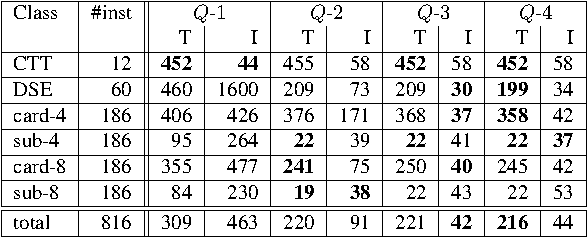
\includegraphics[width=\textwidth]{tables/query_comparison}
\caption{Comparison of different query techniques by runtime and number of solving calls}
\label{tab:query_comparison}
\end{table}

\begin{table}[H]
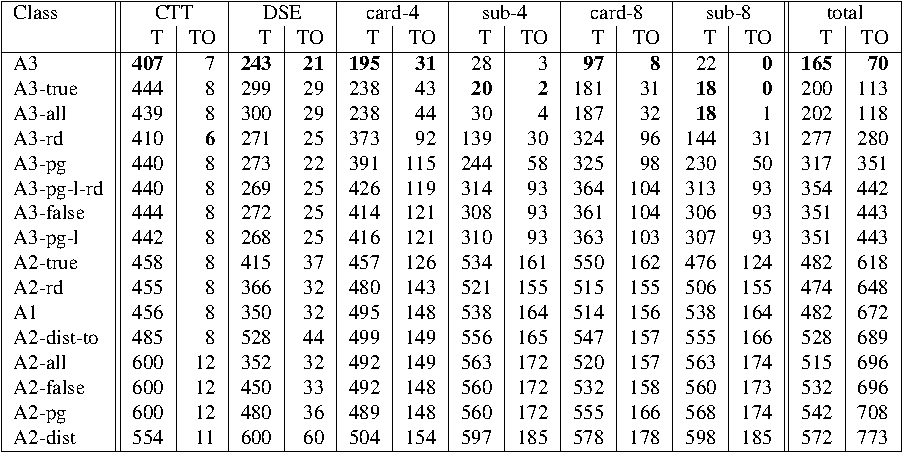
\includegraphics[width=\textwidth]{tables/time_comparison}
\caption{Comparison of approximation techniques by runtime and timeouts}
\label{tab:time_comparison}
\end{table}

\begin{table}[H]
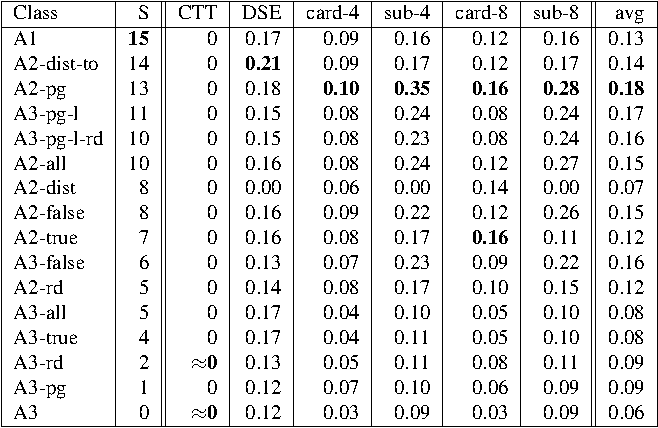
\includegraphics[width=\textwidth]{tables/diverse_comparison}
\caption{Comparison of approximation techniques by diversification quality}
\label{tab:diverse_comparison}
\end{table}

\begin{table}[H]
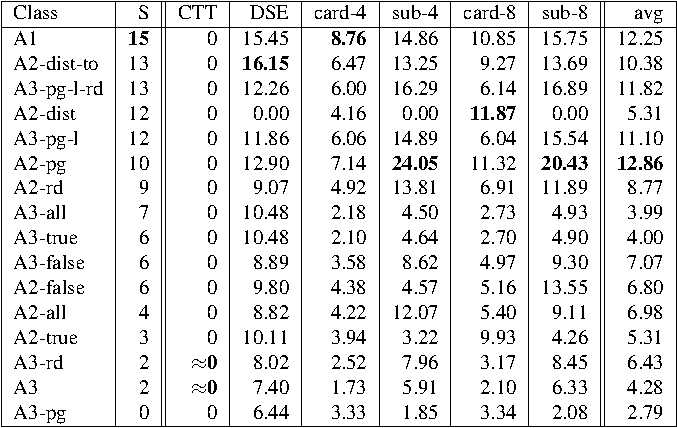
\includegraphics[width=\textwidth]{tables/min_dist_comparison}
\caption{Comparison of approximation techniques by minimum distance}
\label{tab:min_dist_comparison}
\end{table}

\end{document}

%%% Local Variables:
%%% mode: latex
%%% TeX-master: t
%%% End:
